% EPL master thesis covers template
\documentclass{src/1.Cover/EPL-master-thesis-covers-EN}

% Title of the thesis
\title{Accelerating Convolutional Neural Network for FPGA}
% Subtitle - remove this line if not applicable
\subtitle{using Depthwise Separable Convolution and Pruning}

% Name of the student author(s)
\author{Guillaume \textsc{Gheysen}}

\degreetitle{Master [120] in Computer Science and Engineering}

% Name of the supervisor(s)
\supervisor{Jean-Didier \textsc{Legat}}

\secondsupervisor{Christophe \textsc{de Vleeschouwer}}

% Name of the reader(s)
\readerone{Victor \textsc{Joos de Ter Beerst}}
\readertwo{Martin \textsc{Lefèvre}}	 

% Academic year (update if necessary)
\years{2019--2020}

% Acronym
\newacronym{ml}{ML}{Machine Learning}
\newacronym{ai}{AI}{Artificial Intelligence}
\newacronym{nn}{NN}{Neural Networks}
\newacronym{dl}{DL}{Deep Learning}
\newacronym{cnn}{CNN}{Convolutional Neural Network}
\newacronym{cpu}{CPU}{Central Processing Unit}
\newacronym{fpga}{FPGA}{Field-Programmable Gate Array}
\newacronym{gpu}{GPU}{Graphical Processing Unit}
\newacronym{asic}{ASIC}{Application-Specific Integrated Circuit}
\newacronym{dsc}{DSC}{Depthwise Separable Convolution}
\newacronym{fcn}{FCN}{Fully Connected Layer}
\newacronym{pe}{PE}{Processing Element}
\newacronym{fm}{FM}{Feature Map}
\newacronym{gemm}{GEMM}{General Matrix Multiplication}
\newacronym{fft}{FFT}{Fast Fourier Transform}
\newacronym{dsp}{DSP}{Digital Signal Processing}
\newacronym{moc}{MoC}{Model of Computation}
\newacronym{fifo}{FIFO}{First-in First-out}
\newacronym{simd}{SIMD}{Single Instruction Multiple Data}
\newacronym{dram}{DRAM}{Dynamic Random Access Memory}
\newacronym{nas}{NAS}{Neural Architectural Search}
\newacronym{mac}{MaC}{Multiply-and-Accumulate}
\newacronym{oad}{OaA}{Overlap-and-Add}
\newacronym{hdl}{HDL}{Hardware Description Language}
\newacronym{le}{LE}{logic element}
\newacronym{clb}{CLB}{configurable logic block}
\newacronym{ioe}{IOE}{input/output elements}
% Graphic path
\graphicspath{{Images/}}

% Document
\begin{document}
  	% Front cover page
	\maketitle
	\pagenumbering{gobble}
	
	%% Abstract
	\topskip0pt
\vspace*{\fill}
\begin{center}
    \huge{\textsc{Abstract}}
    \end{center}
    
    CNN are powerfull models used in image classification, speech recognition, medical image analysis, etc. However, those models requires a large number of parameters and operations to be executed. Therfore, GPUs are the dominant platform to implement a CNN thanks to their huge computational resources and memory. However, such platforms are power hungry and limit the implementation of CNN on mobile and embedded devices. A solution would be to use, rather than GPU, FPGA which are more energy efficient. However, the FPGA does not require enough resources to implement to most performing models. Therfore, this thesis aims at combining the advantages of two optimizations, pruning and depthwise separable convolution, to further reduce the number of parameters and operations required by a CNN. The performance of this new pruning scheme is studied by implementing such model on FPGA.
\vspace*{\fill}
\afterpage{\blankpage}
\newpage

	
	%% Acknowledgments
	\topskip0pt
\vspace*{\fill}
\begin{center}
    \huge{\textsc{Acknowledgments}}
    \end{center}
    
    I would like to acknowledge the help of some people who were crucial for the completion of this thesis.
    
    First I would like to thank my two supervisors: Prof. Jean-Didier Legat and Prof. Christophe de Vleeschouwer for their support. They provided valuable advice helping me to define the scope of this work and guiding mee through its completion.
    
    Second, I would like to thank the two readers of this thesis: Martin Lefevre and Victor Joos de ter Beerst for devoting their time to read this thesis and asssess my work
    
    Third, I wish to acknowledge the assistance provided by Victor Joos de ter Beerst and Antoine Vanderschueren to accomplish this work which was valuable for me. Their availability to answer my questions was a great help.
    
    Fourth, I would like to thank my family and friends, who were always there to help me when I needed the most. I want also to acknowledge the support of Clara, who was a huge source of inspiration to outdo myself. Moreover, special thanks go to the members of the IngiGang for the time spent during those five years together and the support They provided me.
    
    Finally, I would like to personnally thank all the people who have proofread this thesis, in particular Martine, Julie, Florian, Martin, Maxime, and last but not least Guillaume for giving their precious time to improve the quality of this work. 
\vspace*{\fill}
\afterpage{\blankpage}
\newpage

	
	%% table of contents & figures
	\tableofcontents
	\newpage
	\listoffigures
	\afterpage{\blankpage}
	\newpage
	\printnoidxglossary[type=\acronymtype, title=List of Abrevation, nonumberlist=true, toctitle=List of terms]
	\afterpage{\blankpage}
	\newpage
	
	\pagenumbering{arabic} 
	
	%% Introduction
	\chapter{Introduction}
\section*{Structure of the thesis}
\afterpage{\blankpage}
\newpage
	
	%% Part 1
	% Cnn
    \section{Convolutional Neural Network} \label{sec:cnn}
\acrshort{cnn} is a type of \acrshort{nn} specialized in analyzing visual imagery and natural language processing. \acrshort{cnn}s are feedforward, sparsely connected \acrshort{nn}s, and structured as a pipeline of layers \cite{abdelouahab_accelerating_2018}. It has shown superior performances on different competitions related to Computer Vision and Image Processing \cite{khan_survey_2020}. Nowadays, \acrshort{cnn}s are used in character and gesture recognition, video classification, face detection, etc \cite{shawahna_fpga-based_2019}. This section aims at investigating the different aspects of a \acrshort{cnn}.
%Mand the optimizations that could be made to reduce its size and computational complexity.

First, the building blocks of a CNN are developed in the section \ref{subsec:layer} starting from its basic element \textit{the perceptron}. Then, we describe how to use it to build layers which can perform complex functions. Finally, we detail the other types of layers required to improve the efficiency of the model, such as pooling layer.

Then, section \ref{subsec:models} describes how to effectively combine these layers with a focus on state-of-art networks like AlexNet, VGG16, ResNet, and MobileNetV2.

Finally, Section \ref{subsec:train} focuses on the training of a \acrshort{cnn}. We briefly explain the back-propagation algorithm, which consists of a forward-propagation and a back-propagation.
%
%
\subsection{Structure of a CNN} \label{subsec:layer}
%
A CNN is a pipeline of layers which can be stacked to form a network \cite{abdelouahab_accelerating_2018}. A layer is a high-level building block, which consists of a set of operations, weights, and non-linear functions. The output of one layer can be used as input of the next layer or as the final output of the network. 

This section first introduces the simplest building element of a \acrshort{cnn}: the perceptron. We describe its different components and notably its activation function. Then, we can use this element to build more complex layers such as fully connected and convolutional layer. Finally, we present the pooling layer which it used to reduce the spatial dimensions of the ouput of the previous layer.
%
%
\subsection{Perceptron} \label{subs:perceptron}
The perceptron was first developed in 1957 by \textcite{brain_perceptron_nodate}. It is a computational model based on on the brain. The human brain has a huge number of computing units, \textbf{neurons}. A biological neuron receives information (collects charges) from synapses through chemical mechanisms and once a threshold is passed, the cumulate charges are released (we say the neuro fires) and the information is transmitted to other neurons.

Mathematically, a perceptron has n inputs ($x_1$, ..., $x_n$) which can be expressed as vector \textbf{$\bar{x}$}, n wheights (\textbf{$\bar{w}$}) and a bias \textbf{b}. The perceptron, when receiving an input vector, performs a weighted sum. If the wheighted sum is above a threshold (controlled by the bias which can lower or raise it), the perceptron is 'activated' and outputs a non-zero value (1). The figure \ref{fig:perceptron} illustrates this. We can write the operation in a vector form:
%
$$
h(x| w, b) = h(\sum^{n}_{i=1} x_i \cdot w_i + b) = h ( \textbf{$\bar{w}$}^{T} \textbf{$\bar{x}$} + b)
$$
%
where $h$ is the activation function of the perceptron (the section \ref{subs:acti} describes other activation functions)
$$
h ( \textbf{$\bar{w}$}^{T} \textbf{$\bar{x}$} + b) = \begin{cases} 1, & \mbox{if } \textbf{$\bar{w}$}^{T} \textbf{$\bar{x}$} + b > 0 \\ 0, & \mbox{Otherwise} \end{cases}
$$
In the following section \ref{subs:fcl}, we discover how we can use mutliple perceptrons to create a \textbf{fully-connected layer}.
%
\begin{figure}
    \centering
    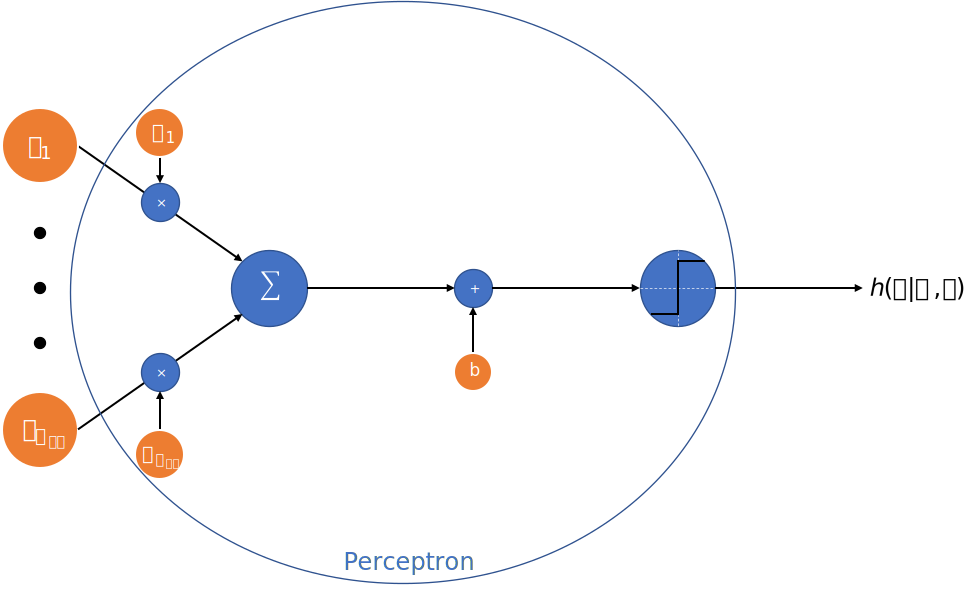
\includegraphics[width=\textwidth]{perceptron.pdf}
    \caption{The Perceptron}
    \label{fig:perceptron}
\end{figure}

%
\subsection{Activation} \label{subs:acti}
The activation function is the non-linear output of the neuron. Its purpose is to decide whether the neuron fires or not. To apply the back-propagation algorithm (see Section \ref{sec:train}), which makes the network learn, we need to have the activation function to be differentiable \cite{lecun_backpropagation_1989}. To optimize the network, we must compute the gradient of the activation function. As the step function described in equation \eqref{eq:step} has a gradient of zero, the perceptron can not learn if we use this activation function. Various activation functions have then been proposed with different properties, as illustrated in Figure \ref{fig:acti}. According to \textcite{khan_survey_2020}, the choice of an appropriate activation function can accelerate the learning phase and some activations have less computational complexity \cite{krizhevsky_imagenet_2012}.
%
\begin{figure}
    \centering
    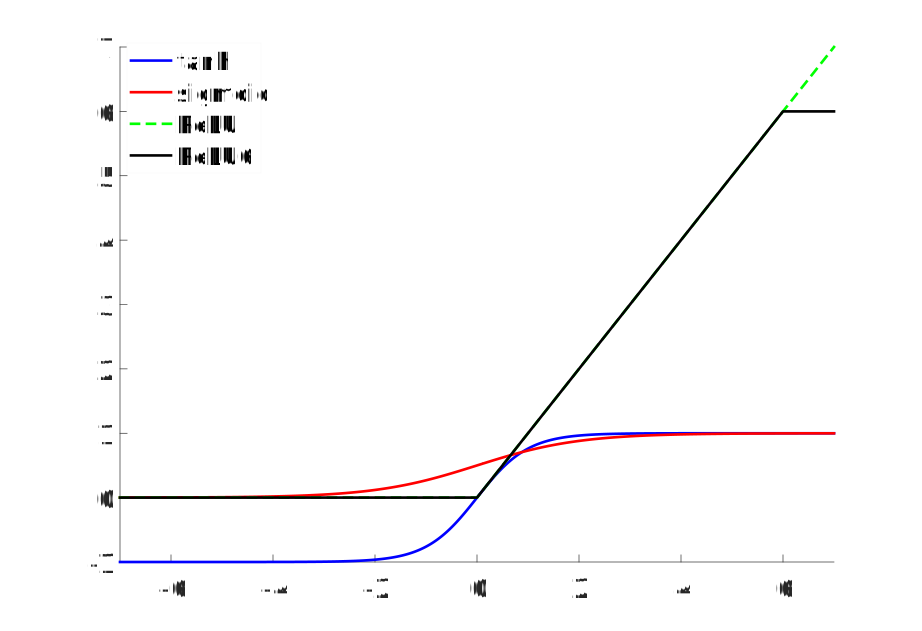
\includegraphics[width=\textwidth]{actifun.pdf}
    \caption{Activation functions}
    \label{fig:acti}
\end{figure}
%
\subsubsection{Sigmoid and Hyperbolic Tangent (Tanh)}
$Sigmoid$ and $Thanh$ are both smooth functions that can be described by equations \eqref{eq:sigmoid} and \eqref{eq:tanh}.
%
\begin{equation}
    h(x) = \frac{1}{1 + e^{-x}}
    \label{eq:sigmoid}
\end{equation}
%
\begin{equation}
    h(x) = \frac{e^{x} - e^{-x}}{e^{x} + e^{-x}}
    \label{eq:tanh}
\end{equation}
%
The two activation functions can be seen in Figure \ref{fig:acti}. They both \textquote{squeeze} the domain $\mathbb{R}$ into a smaller range, $[0, 1]$ for $Sigmoid$, and $[-1, 1]$ for the $Tanh$. However, they also saturate at the asymptotes, which means that often their gradient is close to 0. As the back-propagation algorithm requires gradient multiplication, gradient far away from the output vanishes (close to 0) and deep models do not learn: it is the \textbf{vanishing gradient problem} \cite{goodfellow_deep_2016}.
%
\subsubsection{ReLU}
To solve the problem of saturation, the Rectified Linear Unit (ReLU) has been introduced by \textcite{krizhevsky_imagenet_2012}. Equation \eqref{eq:relu} describes its behavior.
\begin{equation}
    h(x) = max(0, x)
    \label{eq:relu}
\end{equation}
%
This activation function allows faster learning, efficient gradient propagation (no vanishing or exploding gradient), and a faster computation than $Thanh$ or $Sigmoid$. However, it suffers from the \textbf{dying neuron problem} which decreases the model capacity. Some neurons become inactive (output only 0) for essentially all inputs and they \textquote{die}. A neuron that only outputs zero can be discarded. A solution would be to modify the ReLU like leaky ReLU \cite{maas_rectier_2014}, etc.

Other works try to modify the ReLU for implementation on embedded platforms. For example, \cite{howard_mobilenets_2017} uses ReLU6 (equation \eqref{eq:relu6}), which we can see in Figure \ref{fig:acti}. It is designed for fixed-point operations and quantization approaches, instead of floating-point operations which are less efficient in terms of hardware utilization and power consumption (especially on \acrshort{fpga}) \cite{david_hardware_2007}. More information about quantification can be found in Section \ref{subsec:mdopti}. Therefore, if the output $\in [ 0, 6 ]$, the number of bits for the integer part can be limited to 3 bits. We can thus increase the accuracy of the model by assigning the other bits to the decimal part.
%
\begin{equation}
    h(x) = max(0, x, 6)
    \label{eq:relu6}
\end{equation}

%
\subsection{Fully Connected layer} \label{subs:fcl}
The perceptron of Section \ref{subs:perceptron} can be considered as a linear classifier for which the decision boundary is the hyperplane, as seen in equation \eqref{eq:linearclassifer}.
%
\begin{equation}
    b + w_1 \cdot x_1 + ... + w_{n_{in}} \cdot x_{n_{in}} = 0
    \label{eq:linearclassifer}
\end{equation}
%
We can understand why the perceptron is limited because it has only a linear decision boundary. For example, we can implement the AND and OR Boolean functions using a perceptron, but it is impossible to learn the XOR function. To have a non-linear model, we must use a topology of perceptrons. This topology is composed of layers of perceptrons, where each layer, in the case of a \acrshort{cnn}, is called a \textbf{fully-connected layer}. We can see an example in Figure \ref{fig:fcn}.
%
\begin{figure}
    \centering
    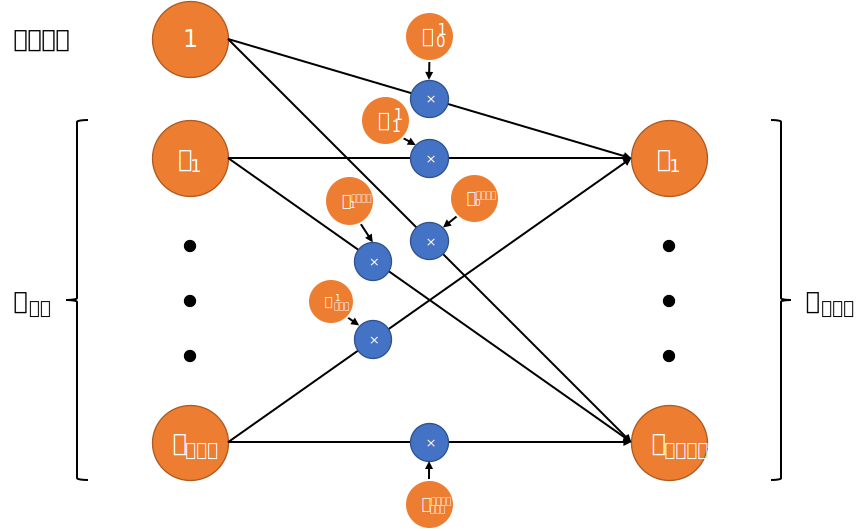
\includegraphics[width=\textwidth]{fcl.pdf}
    \caption{A fully connected layer}
    \label{fig:fcn}
\end{figure}

In the fully-connected layer, each neuron is connected to all the inputs or neurons of previous layers (as the name suggests). As the fully-connected layers are best to make a non-linear classification, we can feed those layers with extracted features, converted as a one-dimension vector \cite{khan_survey_2020}. As a result, usually, the fully-connected layers are placed at the end of \acrshort{cnn}s, where the first layers extract features from the input.

A fully-connected layer is characterized by the number of neurons, activation functions, and the values of weights. The output vector $\boldsymbol{y}$ can be expressed using equation \eqref{eq:fcn}, where $\boldsymbol{x}$ is the vector of the input of the layer and $x_0 = 1$ is the bias;   $\boldsymbol{w}$ is the vector of all the weights of the layer ($w^i_*$ are the weights of the ith perceptron and $w^*_0$ are the biases); $h$ is the activation function of the layer.
%
\begin{equation}
    \boldsymbol{y} = h(\boldsymbol{w}^T \boldsymbol{x}) \qquad \Leftrightarrow \qquad \forall o \in \{ 1, ..., N_{out} \} : y_o = h(\sum^{N_{in}}_{i=0} w^o_i \cdot x_i)
    \label{eq:fcn}
\end{equation}
%
As we have seen that perceptrons can be used to construct a non-linear classifier, we see in the next section \ref{subs:2dconv} the main operation in the \acrshort{cnn}: the \textbf{convolution}, which extracts the feature from input images.

%
\subsection{Convolution layer} \label{subs:2dconv}
A convolutional layer carries out the feature extraction process by applying a set of 3D-convolution filters to a set of input volumes, also called input \acrfull{fm}s. In an \acrshort{cnn}, the first convolutional layers extract low-level features while the deepest one extract more high-level features. The input \acrfull{fm}s are characterized by 3 parameters: \textbf{$N_{ix}$} the width; \textbf{$N_{iy}$} the height; \textbf{$N_{if}$} the depth. An illustration is in figure \ref{fig:notation:ifm}.
The input \acrshort{fm} are then processed with a kernel (of size $N_{kx} \times N_{ky} \times N_{if} \times N_{of}$), that we can see on figure \ref{fig:notation:k}) to obtain the output \acrshort{fm}s. The output \acrshort{fm}s are also characterized by its width $N_{ox}$, its height $N_{oy}$ and its depth $N_{of}$. We can also see a general output \acrshort{fm}s on figure \ref{fig:notation:ofm}.
%
\begin{figure}
    \centering
    %
    \begin{subfigure}{.32\textwidth}
    \centering
    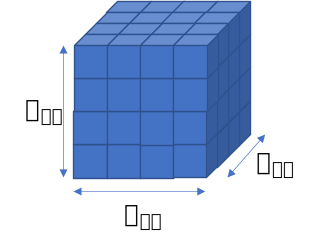
\includegraphics[width=\linewidth]{notifm.pdf}
    \caption{kernel-wise pruning}
    \label{fig:notation:ifm}
    \end{subfigure}
    %
    \begin{subfigure}{.32\textwidth}
    \centering
    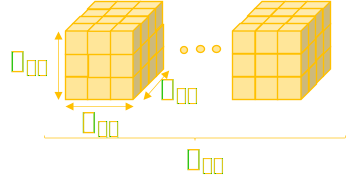
\includegraphics[width=\linewidth]{notk.pdf}
    \caption{Convolution kernel}
    \label{fig:notation:k}
    \end{subfigure}
    %
    \begin{subfigure}{.32\textwidth}
    \centering
    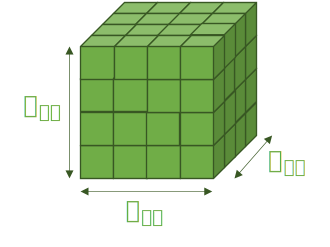
\includegraphics[width=\linewidth]{notofm.pdf}
    \caption{Output \acrshort{fm}s}
    \label{fig:notation:ofm}
    \end{subfigure}
    %
    \caption{Volumes involved in the convolution operations}
    \label{fig:notconv}
\end{figure}

The convolution operation happens as follow. We have an input \acrshort{fm} and a kernel. The kernel acts as a sliding window on the input \acrshort{fm}s. We extract a chunk of pixels of the same size of the kernel in the input \acrshort{fm}. Therefore, we perform a element-wise multiplication with the chunk of data and the kernel to obtain a pixel ouf output. Sliding this kernel on the input \acrshort{fm}s will produce an ouput \acrshort{fm}, where the output pixel at postion $(x, y)$ corresponds to the movement of the sliding window. Since one kernel produces one output \acrshort{fm}, having $N_{of}$ kernels produces then $N_{of}$ output \acrshort{fm}. An illustration of the convolution operation is in figure \ref{}.

Except for $1 \times 1$ kernels, the sliding window can not cover all input pixels and then there is a spatial reduction between the input and output \acrshort{fm}s, while there is an increase in the number of channel. However, we can keep the same dimensions using \textit{padding} on the boundary (for example adding 0).

Moreover, each time the sliding window performs a convolution, it shifts in the input \acrshort{fm}. The amount by which the filter shifts is called the \textit{stride} and it is initialy set to 1. This way we can even more reduce the width and the height of the output \acrshort{fm}s. For example, if we use padding and a stride of 2, $\frac{N_{ix}}{N_{ox}} = \frac{N_{iy}}{N_{oy}} = \frac{1}{2}$ and we use 4 times less pixels.

Finally, we can express the convolution operations mathemalically as in equation \eqref{eq:conv}.
    \begin{multline}
        \forall ox \in \{ 1, ..., N_{ox} \}, oy \in \{ 1, ..., N_{oy} \}, of \in \{ 1, ..., N_{of} \} : \\
        FM_O[ox, oy, oc] = \sum^{N_{if}}_{if=1}
        \sum^{N_{kx}}_{kx=1}
        \sum^{N_{ky}}_{ky=1}
        FM_I[ox \cdot S + kx - \lfloor \frac{N_{kx}}{2} \rfloor,  oy \cdot S + ky - \lfloor \frac{N_{ky}}{2} \rfloor, if] \cdot
        W^{of}_{if}[kx, ky]
        \label{eq:conv}
    \end{multline}

If we compare the convolutional layer with the fully-connected layer, the convolutional layer allows weight sharing and then it needs less weights. For example in AlexNet \cite{krizhevsky_imagenet_2012}, 94\% of the weights are used in the fully-connected layers. But as said earlier, 90\% of the arithmetic operations are done in the convolutional layer.

%
\subsection{Depthwise Separable Convolution}  \label{subs:dsc}
\acrfull{dsc} was first introduced by \textcite{sifre_ecole_2014}. According to \textcite{chollet_xception_2017}, \textquote{\textit{A depthwise separable convolution consists in a \textbf{depthwise convolution}, i.e. a spatial convolution performed independently over each channel of an input, followed by a \textbf{pointwise convolution}, i.e. a $1 \times 1$ convolution, projecting the channel's output by the depthwise convolution onto a new channel space}}.

It means that the \acrshort{dsc} is composed of a depthwise convolution followed by a pointwise convolution as illustrated in Figure \ref{fig:dsc}. This alternative form of convolution has been developed to reduce efficiently the arithmetic complexity, in exchange of a limited loss of accuracy \cite{liu_fpga-based_2019}. As a result, the \acrshort{dsc} has significantly fewer parameters and operations with respect to the standard convolution. Equations \eqref{eq:descopred} and \eqref{eq:descwgred} are used to calculate the reduction factors on weigths and on operations respectively, where $F_{*}$ are the factors of reduction, $W_{sc}$ and $O_{sc}$ are the weights and operations required for a standard convolution, and $W_{dsc}$ and $O_{dsc}$ are the weights and operations required for a \acrshort{dsc} \cite{liu_fpga-based_2019}.
%
\begin{equation}
    F_w = \frac{W_{dsc}}{W_{sc}} =
    \frac{N_{kx} \times N_{ky} \times N_{if} + N_{if} \times N_{of}}{N_{kx} \times N_{ky} \times N_{if} \times N_{of}} =
    \frac{1}{N_{of}} + \frac{1}{N_{kx} \times N_{ky}}
    \label{eq:descopred}
\end{equation}
\begin{equation}
    \begin{split}
        F_o &= \frac{O_{dsc}}{O_{sc}} = \frac{N_{kx} \times N_{ky} \times N_{if} \times N_{ox} \times N_{oy} + N_{if} \times N_{of} \times N_{ox} \times N_{oy}}{N_{kx} \times N_{ky} \times N_{if} \times N_{of} \times N_{ox} \times N_{oy}} \\
        &= \frac{1}{N_{of}} + \frac{1}{N_{kx} \times N_{ky}}
    \end{split}
    \label{eq:descwgred}
\end{equation}

Using equation \eqref{eq:descopred} and equation \eqref{eq:descwgred} and $3 \times 3$ kernels, the reduction of computation and parameters in comparison with the standard convolution is about 9 times \cite{zhang_channel_2019}.
%
\begin{figure}
    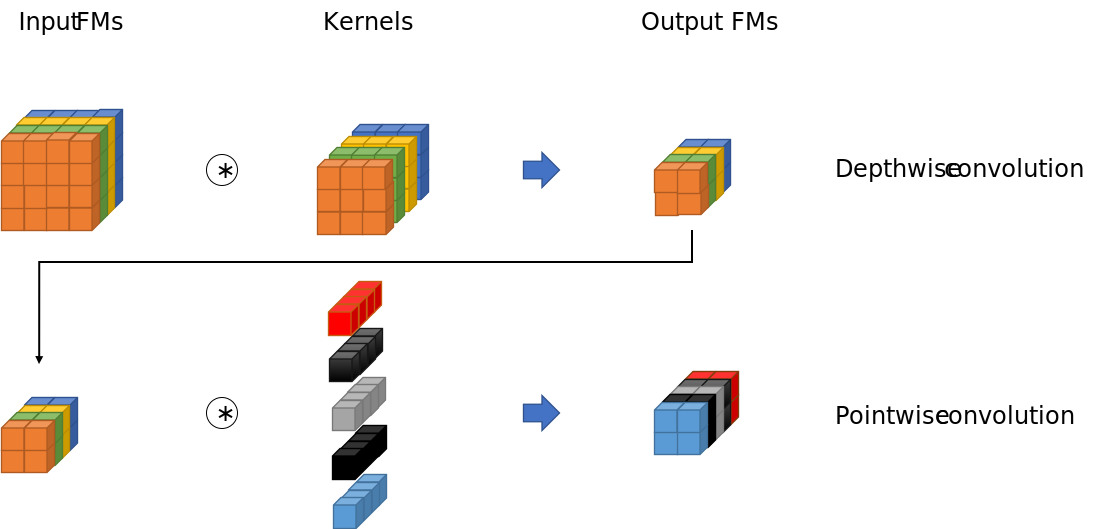
\includegraphics[width=\textwidth]{dsc.pdf}
    \caption{Depthwise Separable Convolution}
    \label{fig:dsc}
\end{figure}

%
\subsection{Pooling} \label{subs:pooling}
Pooling layers are inserted between successive convolutional layer. It aims at reducing the spatial size of each \acrshort{fm}. It reduces the number of parameters and the computation of the network while also increasing the receptive field \cite{shawahna_fpga-based_2019}. The layer divides each \acrshort{fm} in regions of size $K \title K$ and outputs one pixel from each region. This way, we can keep the number of channel and reduce each spatial dimension by $K$.

Various pooling functions can be used, but the most common form is with filters of size $2 \times 2$ where the MAX or AVG operation selects the highest pixel from 4 samples (meaning a reducion 75\%) \cite{suda_throughput-optimized_2016}. An illustration can be found in figure \ref{fig:pool}.
%
\begin{figure}
    \centering
    \includegraphics[width=\textwidth]{pooling.pdf}
    \caption{An example of pooling layers}
    \label{fig:pool}
\end{figure}

%
\subsubsection{Summary}
%
The summary of this section is provided by Figure \ref{fig:layer:summary}. An input image is transmitted to the \acrshort{cnn} then, three different kinds of layers can be used:
%
\begin{enumerate}
    \item The convolutional layer which extract the features from the input.
    \item The pooling layer which summarizes the output of the previous layer.
    \item The fully connected layer which is a non linear classifier.
\end{enumerate}
%
A typical \acrshort{cnn} is composed of two parts, which are built from stacking the previously mentioned layers \cite{matteucci_artificial_2019}:
\begin{enumerate}
    \item The feature extractor part, composed of blocks made of convolutional, activation, and pooling layers.
    \item The classifier part, composed only of fully connected layers.
\end{enumerate}
%
\begin{figure}[H]
    \centering
    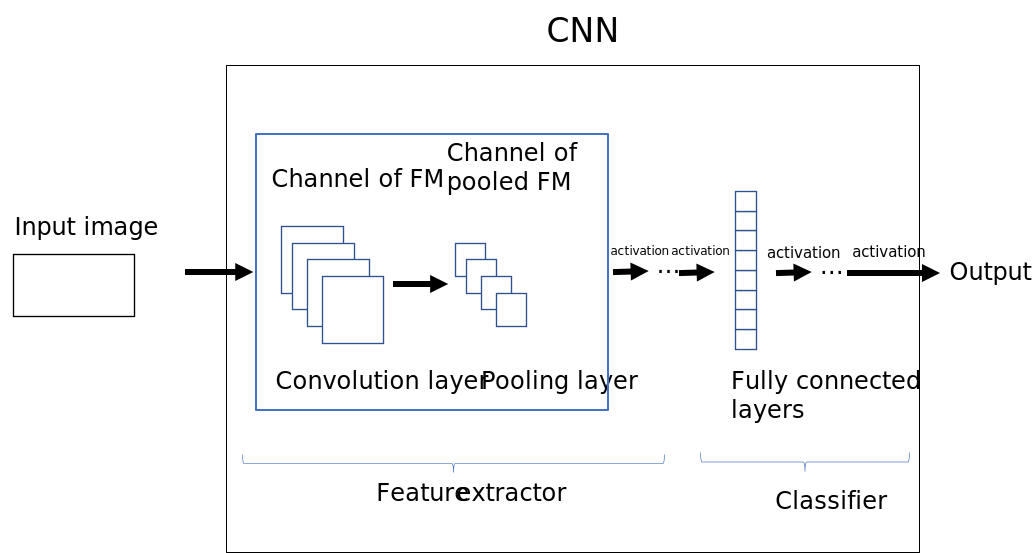
\includegraphics[width=\textwidth]{cnn_summary.pdf}
    \caption{Working principle of a CNN and the different layers which composing it}
    \label{fig:layer:summary}
\end{figure}
%
\subsection{CNN Models} \label{subsec:models}
After the analysis of the CNN structure in Section \ref{subsec:layer}, this section details some of the well-known \acrshort{cnn} networks. They are examples of how to construct an efficient \acrshort{cnn}.

%
\subsection{AlexNet}
AlexNet is a \acrshort{cnn} developed in 2012 by \textcite{krizhevsky_imagenet_2012}. AlexNet has made a breakthrough in the deep \acrshort{cnn} field and this model has won the ImageNet competition. It is made of 5 convolutional layers and 3 fully-connected layers. We can see the network in Figure \ref{fig:alexnet}. Each convolutional layer has a ReLU activation function and it uses pooling.
%
\begin{figure}
    \centering
    \includegraphics[width=\textwidth]{alexnet.pdf}
    \caption{An illustration of the architecture of AlexNet \cite{krizhevsky_imagenet_2012}}
    \label{fig:alexnet}
\end{figure}
%
\subsection{VGG}
After the success of AlexNet, research has been made to have a network with the same accuracy but lower computational complexity. VGG has been introduced by \textcite{simonyan_very_2015} in 2014, which is a deeper variant of AlexNet. It consists of 5 groups of convolutional layers, where the number of layers depends on the version of VGG. It has won the localization and the second-place tracks in the ImageNet challenge in 2014. An illustration can be found in Figure \ref{fig:vgg}. This depth has been possible by using very small ($3 \times 3$) convolution kernels: it allows a larger receptive field while having fewer parameters and more non-linearities than a larger kernel. However, it has a high memory request. We need 100MB per image to be stored in all \acrshort{fm}s for the forward propagation
%
\begin{figure}
    \centering
    \includegraphics[width=\textwidth]{VGG.pdf}
    \caption{An illustration of the architecture of VGG16 \cite{simonyan_very_2015}}
    \label{fig:vgg}
\end{figure}
%
\subsection{ResNet}
Resnet is a very deep network (between 50 and 1000 convolutional layers) proposed by \textcite{he_deep_2015} with more irregular and complex structures compared to the previous networks. \textcite{he_deep_2015} have shown that an increase of the depth does not mean an improvement in the performance of the network and this is not due to overfitting. It is because deeper models are harder to optimize than shallower ones (vanishing gradient). But intuitively, the deeper networks should have at least similar or better performance than shallower models. It is explained by the fact that we can map a deeper model into a shallower one by setting the weights to the identity.

Their solution is to add an \textquote{identify shortcut connection} that skips one or more layers to mitigate the gradient descent problem and try to set the weights to the identity. We can see the process in figure \ref{fig:resnet}. Weights between the skip connection can be used to learn a residual $F(x)$ to improve the solution. The performance of ResNet enables it to be the 2015 ILSVR winner for both localization and classification.
%
\begin{figure}
    \centering
    \includegraphics[width=0.8\textwidth]{resnet.pdf}
    \caption{ResNet building block \cite{he_deep_2015}}
    \label{fig:resnet}
\end{figure}
%
\subsection{MobileNetV2} \label{subs:mbv2}
The drive of the previous networks for accuracy has come for high computational and storage costs which are beyond the capabilities of many mobiles and embedded applications, according to \textcite{cheng_recent_2018}. For the \acrshort{cnn} training phase, it is not a problem thanks to the high performance and large disk and memory storage capacities of the \acrshort{gpu} and \acrshort{cpu} clouds. However, for the inference stage, it is difficult to deploy such networks on mobile devices such as \acrshort{fpga} because of their constraint resources:
%
\begin{itemize}
    \item The enormous computational complexity of \acrshort{cnn}s makes it difficult to deploy on real-time applications and it consumes battery power.
    \item The large number of parameters of \acrshort{cnn}s consumes considerable storage and run-time memory.
\end{itemize}

\textcite{sandler_mobilenetv2_2019} have proposed a network tailored for such constrained environments. To do so, we must first reduce the size and number of operations. They have achieved it using \acrshort{dsc}, introduced in Section \ref{subs:dsc}, and a new kind of layer: inverted residual with a linear bottleneck (observed in Figure \ref{fig:invreslinbot}). It is first composed of a $1 \times 1$ convolution to expand the number of the input \acrshort{fm} channels and then followed by a \acrshort{dsc}. The intermediate increase in the number of channels is supposed to counterbalance the loss of information that occurred by the ReLU. They have also added a skip connection to build a network of great depth, and the last convolution has a linear activation function.
%
\begin{figure}
    \centering
    \includegraphics[width=\textwidth]{mbnv2.pdf}
    \caption{inverted residual with linear bottleneck \cite{sandler_mobilenetv2_2019}}
    \label{fig:invreslinbot}
\end{figure}

%
%
\subsection{Training} \label{subsec:train}
In previous section were described the common building blocks present in \acrshort{cnn} and how to design a \acrshort{cnn}. This section aims at detailing how a network improves automatically its performance for a specific task. This is called \textit{learning}.

The learning phase starts after designing the network. However, before the model can learn, we have to initialize the weights. The most common initialization is random Gaussian distribution \cite{he_delving_2015}. However, the learning phase is affected by the initial values of the weights. If it is too small the network does not learn or if it is too large it might take a very long time to converge. Different initializations were suggested to improve the learning phase: Xavier initialization \cite{glorot_understanding_2010} and He initialization \cite{he_delving_2015}.

When values are assigned to the weights, the backpropagation algorithm can be performed in order to improve the efficiency of the network. The backpropagation algorithm is composed of two steps: the forward pass and the backpropagation. In the following sections we briefly review each of them.
%
\subsection{Forward-propagation} \label{subs:trainforward}
We use the training data as input for the model and we propagate each input through the network using the current weights. The forward propagation produces a vector of output that we can compare with the label of the input (target). This comparison is made with a loss function (for example the mean-square error, that we can see in equation \eqref{eq:mse}). To improve the accuracy of the model, we have to minimize the loss function by finding the optimal weights. This can be done using the algorithms found in the next section \ref{subs:trainbackward}. Moreover, once the model is trained, the inference consists only of the forward propagation.
%
\begin{equation}
    L(\boldsymbol{w}, \boldsymbol{w}) = \sum^{N}_{i=1} (label_i - p(x_i, \boldsymbol{w}))
    \label{eq:mse}
\end{equation}

%
\subsection{Back-propagation} \label{subs:trainbackward}
According to \textcite{ruder_overview_2017}, gradient descent optimization algorithms are the most common one used  to perform optimizations on \acrshort{nn}. These algorithms derive from the idea of gradient descent. As said in the previous section, gradient descent is a way to minimize the loss function in order to parametriz the parameters of the model (weight). Equation \eqref{eq:gd} defines the gradient descent algorithm, where $\eta$ is the learning rate, a positive scalar determining the size of the step in the direction minimizing the gradient \cite{ruder_overview_2017, goodfellow_deep_2016}. If we update the weight in the opposite direction of the gradient, we can reach a local minimum.
%
\begin{equation}
    \boldsymbol{w} = \boldsymbol{w} - \eta \frac{ \partial L( \boldsymbol{x}, \boldsymbol{w} ) }{\partial \boldsymbol{w}}
    \label{eq:gd}
\end{equation}

\textbf{The original gradient descent} or \textbf{batch gradient descent} computes the gradient using the whole dataset (the batch) \cite{ruder_overview_2017, matteucci_artificial_2019}. Equation \eqref{eq:gd-grad} is used to compute this batch gradient. However, this might be impossible to do in practice if the dataset is too large. Indeed, Indeed, the gradient of the whole dataset has to be computed for each update. Therefore, variations of this algorithm have been proposed to make the gradient descent practical.
%
\begin{equation}
    \frac{ \partial L( \boldsymbol{x}, \boldsymbol{w} ) }{\partial \boldsymbol{w}} = \frac{1}{N_{in}} \sum^{Nin}_{i = 0} \frac{ \partial L( x_i, \boldsymbol{w} ) }{\partial \boldsymbol{w}}
    \label{eq:gd-grad}
\end{equation}

\textbf{Stochastic gradient descent}, instead of using the entire dataset, performs the gradient descent algorithm on each training sample of the whole dataset \cite{ruder_overview_2017, matteucci_artificial_2019}. Equation \eqref{eq:sgd-grad} computes the stochastic gradient descent. It avoids the redundant computation of the batch gradient descent. It learns faster and can reach better local minima, however, it is complicated to find the global minimum.
%
\begin{equation}
    \frac{ \partial L( \boldsymbol{x}, \boldsymbol{w} ) }{\partial \boldsymbol{w}} = \frac{ \partial L( x_i, \boldsymbol{w} ) }{\partial \boldsymbol{w}}
    \label{eq:sgd-grad}
\end{equation}

\textbf{Mini-batch gradient descent} is a trade-off between the two previous approaches \cite{ruder_overview_2017, matteucci_artificial_2019}. It performs an update of the weights for every mini-batch of the whole dataset. Equation \eqref{eq:bgd-grad} computes the mini-batch gradient descent, where $N$ is the number of training samples. It shows a better convergence than stochastic gradient descent by reducing the variance and has less computations than batch gradient descent.
%
\begin{equation}
    \frac{ \partial L( \boldsymbol{x}, \boldsymbol{w} ) }{\partial \boldsymbol{w}} = \frac{1}{N} \sum^{N < N_{in}}_{i = 0} \frac{ \partial L( x_i, \boldsymbol{w} ) }{\partial \boldsymbol{w}}
    \label{eq:bgd-grad}
\end{equation}

%
%

    \afterpage{\blankpage}
    \cleardoublepage
    \newpage
% FPGA
    \chapter{FPGA} \label{chap:fpga}
As said at chapter \ref{chap:intr}, the focus is on accelerating the inference stage on \acrshort{fpga}. This chapter reviews the main concepts of the \acrshort{fpga} and its design flows, how to perform the inference stage on the \acrshort{fpga} and the optimizations techniques to improve this inference.
%
%
\section{Concept}
%
%
According to \textcite{harris_digital_2015}, \textit{a \acrfull{fpga} is an array of reconfigurable gates}. It is an a platform that can implement compinatinational and sequential logic, multilevel logic functions. An \acrshort{fpga} also integrate built-in multipliers, high-speed I/Os, data converters, large RAM arrays and processors. \newline \newline
%
An illustration of a general \acrshort{fpga} layout can be found in image \ref{fig:fpga}. An \acrshort{fpga} is an array of configurable \acrfull{le}, also referred as \acrfull{clb}. Each \acrshort{le} can be configured to perform combinational or sequential logic and is connected to other \acrshort{le}s. The \acrshort{le}s array is connected to a set of \acrfull{ioe} to interface with the outside world.\newline \newline
%
A programmer can implement digital designs on the \acrshort{fpga} with a software programming tool, using either an \acrfull{hdl} or a schematic. An \acrshort{hdl} is a language to give the specifications of a digitial design. It allows a faster development cycle than schematic since we work at a higher level of abstraction and the software optimize the gates. The two leading \acrshort{hdl} are \textit{VHDL} and \textit{SystemVerilog}. They are build on the same principles and they mostly differ on the syntax. The final architecture is implemented in \textit{SystemVerilog}.
%
\begin{figure}
    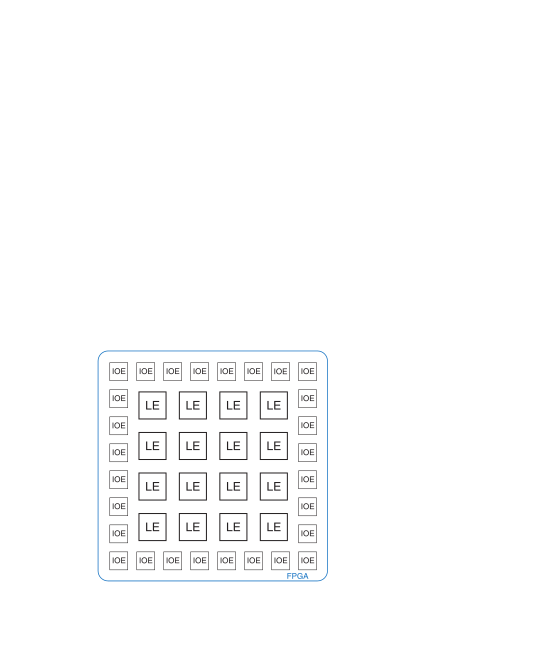
\includegraphics[width=\textwidth]{fpga.pdf}
    \caption{General \acrshort{fpga} layout \cite{harris_digital_2015}}
    \label{fig:fpga}
\end{figure} \newline \newline
%

%
\section{CNN optimizations on FPGA}
%The various optimizations can be grouped into 3 main categories, according to \textcite{abdelouahab_accelerating_2018}:
%\begin{itemize}
%    \item \textbf{Algorithmic Optimizations}: the computational cost of the convolution can be reduced by vectorizing the operation or using faster algorithms. More details can be found in section \ref{subsec:algopti}.
%    \item \textbf{Datapath Optimization}: because of the limited resources on an FPGA, memory is often the bottleneck and optimizing the memory management can increase the throughput. More details can be found in section \ref{subsec:dtptopti}.
%    \item \textbf{\acrshort{cnn} model Optimization}: an important issue of \acrshort{cnn} is their computational complexity and hardware utilization. A solution is then to use approximate computing to trade accuracy for acceleration. This work focus on this category of optimization. More details can be found in section \ref{subsec:mdopti}.
%\end{itemize}
%The following sections introduce and discuss the different optimization approaches and their various techniques.
%%%%%%%%%%%%
\section{Datapath Optimization} \label{sec:dtptopti}
blabla

%
%
\section{CNN inference on FPGA}

    \afterpage{\blankpage}
    \cleardoublepage
    \newpage

	
	%% Part 2
	\chapter{State-of-art} \label{chap:sota}
% inference optimization
\section{CNN optimizations for FPGA} \label{sec:opti_cnn}
%
%
The previous chapter has described the way \acrshort{cnn} work and the different state-of-the-art models. Section \ref{subs:mbv2} evidenced the issue to implement the inference phase on mobile devices such as \acrshort{fpga}. Indeed, the computational complexity and the storage requirements are way beyond their capabilities. This section explores the state-of-the-art approaches to reduce the arithmetic complexity and the hardware utilization to handle this problem on a \acrshort{fpga}. First, Section \ref{subsec:algopti} details how to efficiently handle and optimize the convolution operation on \acrshort{fpga}. Then, Section \ref{subsec:mdopti} covers techniques to reduce the size of the model.
%
\subsection{Algorithmic Optimizations} \label{subsec:algopti}
According to \textcite{shawahna_fpga-based_2019}, 90\% of computation time in \acrshort{cnn} is consumed by the convolution operation. Therefore, decreasing the number of operations in a convolution will reduce the computational complexity of \acrshort{cnn}. This section investigates algorithms that accelerate the convolution operation.
%
%
\subsubsection{GEMM}
%
\acrfull{gemm} is commonly used to process \acrshort{cnn} on \acrshort{cpu} and \acrshort{gpu} \cite{abdelouahab_accelerating_2018}. The \acrshort{gemm} converts the convolution operation as a matrix-vector multiplication. In other words, a mini-batch of input \acrshort{fm} and kernels are transformed into two 2D matrices, as illustrated in Figure \ref{fig:gemm}. It is done in such a way that the multiplication between those two matrices gives the same result as a standard convolution. 
%
\begin{figure}[H]
    \centering
    \includegraphics[width=0.5\textwidth]{gemm.pdf}
    \caption{\acrshort{gemm}-based processing of a standard convolution layer, from \cite{abdelouahab_accelerating_2018}}
    \label{fig:gemm}
\end{figure}
%
The advantage of this method becomes more significant as the size of the mini-batch grows \cite{abdelouahab_accelerating_2018}. However, this approach is not appropriate for \acrshort{fpga}. Indeed, \textcite{zhu_efficient_2020, sze_efficient_2017} pointed out that the \acrshort{fm}s, when converted to a vector, must be copied multiple times. It leads to huge memory storage requirements, memory footprint, and complex memory management access patterns. Furthermore, it does not reduce the arithmetic complexity of the convolution \cite{liang_evaluating_2020}.
%
\subsubsection{Fast algorithms for convolution}
%
%
As mentioned previously, the \acrshort{gemm} can accelerate the convolution but it does not reduce the number of operations. Therefore, we can investigate algorithms that aim at computing the convolution operation with fewer operations, named \textbf{fast convolution algorithms}. According to \textcite{liang_evaluating_2020}, there exist two fast convolution algorithms that perform efficiently the 2D convolution: Winograd minimal filter algorithm and \acrfull{fft}. 

The idea behind these fast convolution algorithms is to transform a kernel and a tile of input into a target domain, where the convolution corresponds to an element-wise multiplication in that domain \cite{abdelouahab_accelerating_2018}. In the end, we can obtain the corresponding tile of output by applying the inverse transformation on the product tile. As a result, the fast algorithm produces a tile of output (rather than a single pixel) and reduces the total number of operations by computing an element-wise multiplication (rather than a multiplication followed by an addition).

Therefore, both fast convolutions can be described by a common formula, as expressed in Equation \eqref{eq:comform}, where $T_o$ (resp. $T_I$) is the output (resp. the input) tile, $K$ is the kernel, $\mathcal{H}$ (resp. $\mathcal{H}^{-1}$) is the domain transformation (resp. the inverse transformation) required to perform the algorithms and $\odot$ is the element-wise multiplication \cite{liang_evaluating_2020}.
%
\begin{equation}
    T_O = \mathcal{H}^{-1} [ \ \mathcal{H}(T_I) \ \odot \ \mathcal{H}(K) \ ]
    \label{eq:comform}
\end{equation}
%
\subsubsection{Winograd-based convolution}
%
The Winograd minimal filter algorithm was first introduced by \cite{winograd_arithmetic_1980}. According to Equation \eqref{eq:comform} and \textcite{abdelouahab_accelerating_2018}, the algorithm can be defined using the following steps:
\begin{itemize}
    \item An input \acrshort{fm} tile $g$ of size $(T_{ix} \times T_{iy})$ is pre-processed: $$\mathcal{H}(T_I) = \boldsymbol{G^{T}} T_I \boldsymbol{G} $$
    \item In the same way, the kernel $K$, of size $(K_x \times K_y)$ is also transformed: $$\mathcal{H}(K) = \boldsymbol{B^{T}} K \boldsymbol{B}$$
    \item The inverse transformation function is then applied to obtain the output tile: $$\mathcal{H}^{-1}(E) = \boldsymbol{A^{T}} E \boldsymbol{G}$$ Where $E$ is the result of the element-wise multiplication of the two transformed tiles. $$ E = \mathcal{H}(T_I) \ \odot \ \mathcal{H}(K) $$
\end{itemize}
As a result, the output tile $T_O$, of the Winograd Filtering algorithm denoted $F(T_{ix} \times T_{iy}, K_x \times K_y)$, is computed using Equation \eqref{eqn:winograd} \cite{winograd_arithmetic_1980}. The advantage of using the Winograd-based convolution is that the transformation matrix $\boldsymbol{G}$, $\boldsymbol{B}$, $\boldsymbol{A}$ can be computed off-line once $(T_{ix}, T_{iy}, K_x, K_y)$ are fixed, using the Winograd Algorithm \cite{winograd_arithmetic_1980}. Therefore, these domain transform operations become multiplications with a constant and can be optimized on \acrshort{fpga} \cite{liang_evaluating_2020}.
%
\begin{equation}
    T_O = \boldsymbol{A^{T}} [ \ \boldsymbol{G^{T}} T_I \boldsymbol{G} \odot \boldsymbol{B^{T}} K\boldsymbol{B} \ ] \boldsymbol{A}
    \label{eqn:winograd}
\end{equation}

According to \textcite{winograd_arithmetic_1980}, the Winograd convolution reduces the number of multiplications at the cost of an increase in the numbers of additions. The gain obtained is defined in Equation \eqref{eq:winograd_gain} \cite{winograd_arithmetic_1980}. For example, if $T_{ix} = T_{iy} = 2$ and $N_{kx} = N_{ky} = 3$, the complexity reduction factor $F_{multiplication}$ equals $2.25$ \cite{lavin_fast_2016}.
%
\begin{equation}
    F_{multiplication} = \frac{T_{ix} \times T_{iy} \times N_{kx} \times N_{ky}}{(T_{ix} + N_{kx} - 1) \times (T_{iy} + N_{ky} - 1)}
    \label{eq:winograd_gain}
\end{equation}
%
\subsubsection{FFT-based convolution}
%
The \acrshort{fft}, introduced by \textcite{cooley_algorithm_1965}, is an algorithm used to compute the discrete Fourier transform. As presented earlier, once the tile and kernel are in the frequency-domain, the operation corresponding to the convolution is the element-wise multiplication. Therefore, we can use the \acrshort{fft} to perform the convolution operation described in Equation \eqref{eq:comform}, where \cite{liang_evaluating_2020}:
\begin{itemize}
    \item $\mathcal{H}(*) = FFT(*)$
    \item $\mathcal{H}^{-1}(*) = IFFT(*)$
\end{itemize}
%
Using \acrshort{fft}, the computational complexity factor can be reduced from $O(N_{ix} \times N_{iy} \times N_{kx} \times N_{ky})$ to $O(N_{i\{x,y\}} log_2(N_{k\{x,y\}}))$ \cite{w_smith_scientist_1997}.
%
\subsubsection{Comparison between the two fast convolution algorithms}
%
Winograd-based convolution seems to be a preferred way to perform fast convolution. Indeed, \textcite{lavin_fast_2016} demonstrated that Winograd convolution is more efficient when the kernel and the stride are small ($K_* \leq 3$ for the kernel) while \acrshort{fft}-based convolution is more adequate when the kernel is large \cite{ahmad_towards_2019, chitsaz_acceleration_2020}. However, current \acrshort{cnn} trends use small kernels \cite{sandler_mobilenetv2_2018, liang_evaluating_2020} and so, the Winograd convolution.

Moreover, there are examples of successful \acrshort{fpga} implementations of Winograd algorithm: \textcite{liang_evaluating_2020, aydonat_opencl_2017} used Winograd transform and reduced their computational complexity by around 50\%. However, the Winograd algorithm also increased bandwidth utilization \cite{xiao_exploring_2017}.

Yet, \textcite{liang_evaluating_2020, chitsaz_acceleration_2020, zeng_optimizing_2017} worked on the optimization of the frequency-domain convolution on \acrshort{fpga} with small filter by using \acrfull{oad} technique \cite{w_smith_scientist_1997} to lower the number of operations and increase the data parallelism. However, according to \textcite{liang_evaluating_2020, podili_fast_2017}, \acrshort{fft}-based convolution still requires more memory, bandwidth, and logic resources (additions and multiplications) than Winograd. Furthermore, \textcite{zhang_caffeine_2016} pointed out that performing \acrshort{fft} convolution with $1 \times 1$ kernel is inefficient, and they performed it in time-domain only.

%
\section{Model Optimizations} \label{sec:mdopti}
blabla


%
\chapter{Accelerating \acrshort{cnn} inference on \acrshort{fpga}}
\label{chap:inf}
As said at chapter \ref{chap:intr}, interest has been made on accelerating the inference phase on \acrshort{fpga}. This chapter reviews the acceleration approaches to perform an efficient inference. \newline \newline
The three main optimization can be categorized according to \cite{abdelouahab_accelerating_2018}:
\begin{itemize}
    \item \textbf{Algorithmic Optimizations}: the computational cost of the convolution can be reduced by vectorizing them. More details can be found in section \ref{sec:algopti}.
    \item \textbf{Datapath Optimization}: because of the limited resources on a \acrshort{fpga}, memory if often the bottleneck and optimizing the memory management can increase the throughput. More details can be found in section \ref{sec:dtptopti}.
    \item \textbf{\acrshort{cnn} model Optimization}: an important issue of \acrshort{cnn} is their computational complexity and their hardware utilization. A solution is then to use approximate computing and trade accury for acceleration. This work focus on this kind of optimization. More details can be found in section \ref{sec:mdopti}.
\end{itemize}
The following sections introduce and discuss the different optimizations. Then we compare the most relevant approaches on \acrshort{fpga} on section \ref{sec:cclopti}.
%%%%%%%%%%%%
\subsection{Algorithmic Optimizations} \label{subsec:algopti}
According to \textcite{shawahna_fpga-based_2019}, 90\% of computation time in \acrshort{cnn} is consumed by the convolution operation. Therefore, decreasing the number of operations in a convolution will reduce the computational complexity of \acrshort{cnn}. This section investigates algorithms that accelerate the convolution operation.
%
%
\subsubsection{GEMM}
%
\acrfull{gemm} is commonly used to process \acrshort{cnn} on \acrshort{cpu} and \acrshort{gpu} \cite{abdelouahab_accelerating_2018}. The \acrshort{gemm} converts the convolution operation as a matrix-vector multiplication. In other words, a mini-batch of input \acrshort{fm} and kernels are transformed into two 2D matrices, as illustrated in Figure \ref{fig:gemm}. It is done in such a way that the multiplication between those two matrices gives the same result as a standard convolution. 
%
\begin{figure}[H]
    \centering
    \includegraphics[width=0.5\textwidth]{gemm.pdf}
    \caption{\acrshort{gemm}-based processing of a standard convolution layer, from \cite{abdelouahab_accelerating_2018}}
    \label{fig:gemm}
\end{figure}
%
The advantage of this method becomes more significant as the size of the mini-batch grows \cite{abdelouahab_accelerating_2018}. However, this approach is not appropriate for \acrshort{fpga}. Indeed, \textcite{zhu_efficient_2020, sze_efficient_2017} pointed out that the \acrshort{fm}s, when converted to a vector, must be copied multiple times. It leads to huge memory storage requirements, memory footprint, and complex memory management access patterns. Furthermore, it does not reduce the arithmetic complexity of the convolution \cite{liang_evaluating_2020}.
%
\subsubsection{Fast algorithms for convolution}
%
%
As mentioned previously, the \acrshort{gemm} can accelerate the convolution but it does not reduce the number of operations. Therefore, we can investigate algorithms that aim at computing the convolution operation with fewer operations, named \textbf{fast convolution algorithms}. According to \textcite{liang_evaluating_2020}, there exist two fast convolution algorithms that perform efficiently the 2D convolution: Winograd minimal filter algorithm and \acrfull{fft}. 

The idea behind these fast convolution algorithms is to transform a kernel and a tile of input into a target domain, where the convolution corresponds to an element-wise multiplication in that domain \cite{abdelouahab_accelerating_2018}. In the end, we can obtain the corresponding tile of output by applying the inverse transformation on the product tile. As a result, the fast algorithm produces a tile of output (rather than a single pixel) and reduces the total number of operations by computing an element-wise multiplication (rather than a multiplication followed by an addition).

Therefore, both fast convolutions can be described by a common formula, as expressed in Equation \eqref{eq:comform}, where $T_o$ (resp. $T_I$) is the output (resp. the input) tile, $K$ is the kernel, $\mathcal{H}$ (resp. $\mathcal{H}^{-1}$) is the domain transformation (resp. the inverse transformation) required to perform the algorithms and $\odot$ is the element-wise multiplication \cite{liang_evaluating_2020}.
%
\begin{equation}
    T_O = \mathcal{H}^{-1} [ \ \mathcal{H}(T_I) \ \odot \ \mathcal{H}(K) \ ]
    \label{eq:comform}
\end{equation}
%
\subsubsection{Winograd-based convolution}
%
The Winograd minimal filter algorithm was first introduced by \cite{winograd_arithmetic_1980}. According to Equation \eqref{eq:comform} and \textcite{abdelouahab_accelerating_2018}, the algorithm can be defined using the following steps:
\begin{itemize}
    \item An input \acrshort{fm} tile $g$ of size $(T_{ix} \times T_{iy})$ is pre-processed: $$\mathcal{H}(T_I) = \boldsymbol{G^{T}} T_I \boldsymbol{G} $$
    \item In the same way, the kernel $K$, of size $(K_x \times K_y)$ is also transformed: $$\mathcal{H}(K) = \boldsymbol{B^{T}} K \boldsymbol{B}$$
    \item The inverse transformation function is then applied to obtain the output tile: $$\mathcal{H}^{-1}(E) = \boldsymbol{A^{T}} E \boldsymbol{G}$$ Where $E$ is the result of the element-wise multiplication of the two transformed tiles. $$ E = \mathcal{H}(T_I) \ \odot \ \mathcal{H}(K) $$
\end{itemize}
As a result, the output tile $T_O$, of the Winograd Filtering algorithm denoted $F(T_{ix} \times T_{iy}, K_x \times K_y)$, is computed using Equation \eqref{eqn:winograd} \cite{winograd_arithmetic_1980}. The advantage of using the Winograd-based convolution is that the transformation matrix $\boldsymbol{G}$, $\boldsymbol{B}$, $\boldsymbol{A}$ can be computed off-line once $(T_{ix}, T_{iy}, K_x, K_y)$ are fixed, using the Winograd Algorithm \cite{winograd_arithmetic_1980}. Therefore, these domain transform operations become multiplications with a constant and can be optimized on \acrshort{fpga} \cite{liang_evaluating_2020}.
%
\begin{equation}
    T_O = \boldsymbol{A^{T}} [ \ \boldsymbol{G^{T}} T_I \boldsymbol{G} \odot \boldsymbol{B^{T}} K\boldsymbol{B} \ ] \boldsymbol{A}
    \label{eqn:winograd}
\end{equation}

According to \textcite{winograd_arithmetic_1980}, the Winograd convolution reduces the number of multiplications at the cost of an increase in the numbers of additions. The gain obtained is defined in Equation \eqref{eq:winograd_gain} \cite{winograd_arithmetic_1980}. For example, if $T_{ix} = T_{iy} = 2$ and $N_{kx} = N_{ky} = 3$, the complexity reduction factor $F_{multiplication}$ equals $2.25$ \cite{lavin_fast_2016}.
%
\begin{equation}
    F_{multiplication} = \frac{T_{ix} \times T_{iy} \times N_{kx} \times N_{ky}}{(T_{ix} + N_{kx} - 1) \times (T_{iy} + N_{ky} - 1)}
    \label{eq:winograd_gain}
\end{equation}
%
\subsubsection{FFT-based convolution}
%
The \acrshort{fft}, introduced by \textcite{cooley_algorithm_1965}, is an algorithm used to compute the discrete Fourier transform. As presented earlier, once the tile and kernel are in the frequency-domain, the operation corresponding to the convolution is the element-wise multiplication. Therefore, we can use the \acrshort{fft} to perform the convolution operation described in Equation \eqref{eq:comform}, where \cite{liang_evaluating_2020}:
\begin{itemize}
    \item $\mathcal{H}(*) = FFT(*)$
    \item $\mathcal{H}^{-1}(*) = IFFT(*)$
\end{itemize}
%
Using \acrshort{fft}, the computational complexity factor can be reduced from $O(N_{ix} \times N_{iy} \times N_{kx} \times N_{ky})$ to $O(N_{i\{x,y\}} log_2(N_{k\{x,y\}}))$ \cite{w_smith_scientist_1997}.
%
\subsubsection{Comparison between the two fast convolution algorithms}
%
Winograd-based convolution seems to be a preferred way to perform fast convolution. Indeed, \textcite{lavin_fast_2016} demonstrated that Winograd convolution is more efficient when the kernel and the stride are small ($K_* \leq 3$ for the kernel) while \acrshort{fft}-based convolution is more adequate when the kernel is large \cite{ahmad_towards_2019, chitsaz_acceleration_2020}. However, current \acrshort{cnn} trends use small kernels \cite{sandler_mobilenetv2_2018, liang_evaluating_2020} and so, the Winograd convolution.

Moreover, there are examples of successful \acrshort{fpga} implementations of Winograd algorithm: \textcite{liang_evaluating_2020, aydonat_opencl_2017} used Winograd transform and reduced their computational complexity by around 50\%. However, the Winograd algorithm also increased bandwidth utilization \cite{xiao_exploring_2017}.

Yet, \textcite{liang_evaluating_2020, chitsaz_acceleration_2020, zeng_optimizing_2017} worked on the optimization of the frequency-domain convolution on \acrshort{fpga} with small filter by using \acrfull{oad} technique \cite{w_smith_scientist_1997} to lower the number of operations and increase the data parallelism. However, according to \textcite{liang_evaluating_2020, podili_fast_2017}, \acrshort{fft}-based convolution still requires more memory, bandwidth, and logic resources (additions and multiplications) than Winograd. Furthermore, \textcite{zhang_caffeine_2016} pointed out that performing \acrshort{fft} convolution with $1 \times 1$ kernel is inefficient, and they performed it in time-domain only.

%%%%%%%%%%%%
\section{Datapath Optimization} \label{sec:dtptopti}
blabla

%%%%%%%%%%%%
\section{Model Optimizations} \label{sec:mdopti}
blabla

%%%%%%%%%%%%
\section{Conclusion} \label{sec:cclopti}
We can observe on table that pruning seem to be a preferable solutions because ... \newline \newline
On next chapter we are going to explore how to handle pruning on \acrshort{fpga}.


%

\fbox{\parbox{ \linewidth \fboxrule \fboxsep }{ \textbf{Conclusion about the background}:

\vspace{5mm}
We have seen in this chapter what is a \acrshort{cnn}, how to build, and train it. We have also seen that the most performing models have a huge computational complexity and memory utilization, which limit the implementation of such models on mobile platforms, such as \acrshort{fpga}. Different approaches can be explored such as fast convolutions algorithms. But they only reduce the computational complexity while increasing hardware utilization. Therefore, pruning and model designs seem to be promising optimizations because they both aim at reducing those problems. Therefore, this work focus on the use of both approaches to see if their gain can be combined. To show our results, we apply pruning on MobileNetV2. As quantizing is an orthogonal approach to pruning, we also use 16-bit fixed-point formats because the loss of accuracy can be controlled.
}}
\afterpage{\blankpage}
\cleardoublepage
\newpage

	
	%% Part 3
	\chapter{Accelerating Convolutional Neural Networks for FPGA using Depthwise Separable Convolution and Pruning} \label{chap:pratique}
%
%
In the previous chapter, we introduced pruning, which reduces both size and computational complexity of \acrshort{cnn}s. We also showed that there exist various pruning schemes. Each of them can be categorized from coarse-grained to fine-grained. Coarse-grained pruning schemes have the advantage that they can be easily implemented on \acrshort{gpu} and \acrshort{cpu} in exchange for a drop of accuracy. On the other hand, fine-grained pruning schemes can limit this reduction of accuracy but can create irregular access pattern that makes them difficult to implement on such platforms. 

To have an efficient \acrshort{fpga}-based accelerator, we should focus on implementing the most fine-grained pruning scheme possible to apply a high sparsity while limiting the loss of accuracy. This shows the advantage of using \acrshort{fpga} accelerator because, as said previously, this type of pruning scheme is not easily implementable on \acrshort{cpu} and \acrshort{gpu}

In this chapter, we define an \acrshort{fpga}-based accelerator architecture that integrates both pruning and \acrshort{dsc} (see Section \ref{subs:dsc}) to reduce the number of weights and operations. To show its applicability, this architecture implements a state-of-the-art network that includes \acrshort{dsc} and targets an embedded platform: MobileNetV2 (Sections \ref{subs:mbv2} and \ref{subsec:mdopti}). Since the pruning can cause degradation of the performance, we have to determine the design objectives of the architecture and its associated pruning scheme, which are the following:
%
\begin{enumerate}
    \item The pruning scheme is as fine-grained as possible.
    \item The pruning scheme reduces the computational complexity.
    \item The pruning scheme allows for a reduction of the memory required to store the weights.
    \item The proposed architecture provides a logically correct output.
    \item An increase in the sparsity improves the performance of the architecture.
\end{enumerate}

Moreover, the \acrshort{fpga}-based accelerator architecture is implemented on a Cyclone V \acrshort{fpga}.

Section \ref{sec:design} aims at developing the pruning scheme and the algorithm to handle it. We also define in this section the weight and operation reduction factors obtained when applying the proposed pruning scheme. We also define a weight compressed format to reduce weight memory use. We then perform a loop analysis on the proposed algorithm to determine the optimal hardware design variables and the structure of the architecture.

Section \ref{sec:implementation} describes the implementation of the \acrshort{fpga}-based accelerator architecture and details its dataflow. We start by explaining the overall architecture and then we go in more details into each of its components.

Section \ref{sec:measure} shows the results obtained and discusses if the proposed design objectives are met.
%
\section{Design of an FPGA-based accelerator integrating structured sparse DSC} \label{sec:design}
As previously said,  the aim of this section is to develop a pruning scheme for \acrshort{cnn} model (MobileNetV2) and a dataflow able to support it. First we details the pruning scheme used and the gain obtained by applying the pruning. 
%
\subsection{Pruning scheme} \label{subsec:pscheme}
%
\acrshort{dsc} is composed of two types of convolution: depthwise and pointwise convolution. We have decided to apply pruning on the pointwise filters for various reasons:
%
\begin{itemize}
    \item In MobileNet and MobileNetV2, most of the operations are done in the pointwise convolutions \cite{zhang_channel_2019, tu_pruning_2019}.
    \item As each kernel of pointwise kernel, is a vector of size $1 \times 1  \times Nif$. It means that we have to prune in the axis of the channel and apply the same scheme as \textcite{kang_accelerator-aware_2020}.
    \item As in MobileNetV2, each \acrshort{dsc} follows a $1 \times 1$ convolution, we can apply the pruning scheme to every $1 \times 1$ convolutions in the network.
\end{itemize}
%
As mentionned above, we can develop a pruning scheme that is inspired by the methodology of \textcite{kang_accelerator-aware_2020} which performs an channel-axis pruning. Ideally, without pruning, each \acrshort{pe} performing a pointwise convolution, fetches $N_{if}$ weights and their corresponding input pixels (pointwise convolution only convolve pixels in the channel-axis). Then each non-pruned weight is convolved with its corresponding pixel. However, as the resource of the \acrshort{fpga} are limited, the \acrshort{pe} can load $N_{par} \leq N_{if}$ weights and pixels.

%
\begin{figure}
    \centering
    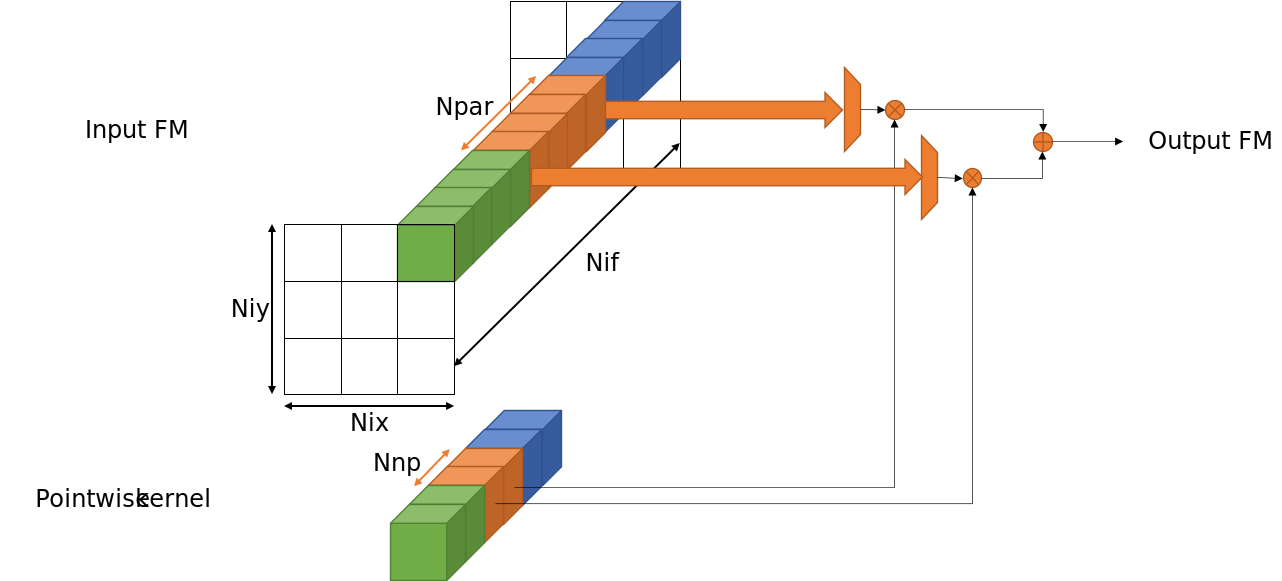
\includegraphics[width=\textwidth]{pruningscheme.pdf}
    \caption{Process of convolution with a sparse pointwise kernel, inspired from \cite{kang_accelerator-aware_2020}}
    \label{fig:prunedwg}
\end{figure}
%
As pointed out by \cite{kang_accelerator-aware_2020}, the unstructured pruning of the pointwise kernel can cause several issues. First, it can causes misalignement between the weight and pixel fetching group. Indeed if we prune the first $N_{par}$ weights in the kernel, the first pixels fetching is useless. Second, there can be a load-imbalance problem that can occur between two \acrshort{pe}s if the number of weights between the two kernels is different. To solve these problems, the solution proposed by \cite{kang_accelerator-aware_2020} is to allign fetching groups of size $N_{par}$, and for each weight fetching group keep a uniform number of weights called $N_{np}$, as illustrated in Figure \ref{fig:prunedwg}. Therefore, it solves also the load imballance problem and can be applied to every $1 \times 1$ kernels.

%
\begin{table}
    \center
    \begin{tabular}{|c|c|c|}
        \hline
        $N_{par}$ & The input pixel fetching group size. & $N_{par} \leq N_{if}$ \\
        \hline
        $N_{np}$  & The pointwise weight fetching group size. & $N_{np} \leq N_{par}$ \\
        \hline
        $N_{gr}$  & The number of fetching groups & $N_{gr} = \left\lceil \frac{N_{if}}{N_{par}} \right\rceil $ \\
        \hline
        $\alpha$  & The pruning ratio & $\alpha = \frac{N_{np}}{N_{par}}  $ \\
        \hline
    \end{tabular}
    \caption{Pruning parameters}
    \label{tab:pr_param}
\end{table}
%
To summarise, each depthwise kernel is composed of $N_{gr}$ weight fetching groups of $N_{np}$ weights, where each group corresponds to a pixels fetching group of size $N_{par}$. We should add that this pruning scheme is not the same as \textit{channel pruning} since we do not constraint the same weights to be pruned in each group. Therefore, I have not considered the pruning of the pointwise filter associated with the pruning of a weight in each kernels. The pruning parameters are defined in Table \ref{tab:pr_param}.
%
\subsubsection{Reduction factor}
%
We can now evaluate the reduction factor of the \acrshort{dsc} including pruning with respect to the \acrshort{dsc} without pruning and the standard convolution. Considering the size of the input feature map of the pointwise convolution is $N_{ix}  \times N_{iy} \times N_{if}$, the size of the depthwise filter is $N_{kx} \times N_{ky} \times N_{if}$, the size of the non-pruned pointwise convolution $N_{if} \times N_{of}$, the fetching group size is $N_{par}$, and the number of pruned weights is $N_{np}$. The amount of weights $W_{DSC}$ and operations $O_{DSC}$ of the \acrshort{dsc} can be determined using Equation \eqref{eq:dsc_wg_op} \cite{bai_cnn_2018, liu_fpga-based_2019}.
%
\begin{align}
    W_{DSC} &= N_{kx} \times N_{ky} \times N_{if} + N_{if} + \times N_{of}\\
    O_{DSC} &= N_{ix} \times N_{iy} \times N_{kx} \times N_{ky} \times N_{if} + N_{ix} \times N_{iy} \times N_{if} \times N_{of}
    \label{eq:dsc_wg_op}
\end{align}
%
The same way, the amount of weights $W_{PR_DSC}$ and operations $O_{PR_DSC}$ of the \acrshort{dsc} with pruning can be determined using Equation \eqref{eq:pr_dsc_pr_wg_op}.
%
\begin{align}
    W_{PR_DSC} &= N_{kx} \times N_{ky} \times N_{if} + \times N_{if} + N_{np} \times N_{gr} \times N_{of}\\
    O_{PR_DSC} &= N_{ix} \times N_{iy} \times N_{kx} \times N_{ky} \times N_{if} + N_{ix} \times N_{iy} \times N_{gr} \times N_{np} \times N_{of} 
    \label{eq:pr_dsc_wg_op}
\end{align}
%
Thus, the reduction factor on weights $F_{Wg}$ and operations $F_{Op}$ can be calculated in Equation \eqref{eq:factor_comp}. More information about the demonstration to find the relations can be found in Appendix \ref{appendix:factor}.
%
\begin{align}
    F_{Wg} &= \frac{1 + \frac{N_{kx} \times N_{ky}} {N_{of}}} {\alpha + \frac{N_{kx} \times N_{ky}} {N_{of}}}\\
    F_{Op} &= \frac{1 + \frac{N_{kx} \times N_{ky}} {N_{of}}} {\alpha + \frac{N_{kx} \times N_{ky}} {N_{of}}}
    \label{eq:factor_comp}
\end{align}
%
\begin{figure}
    \centering
    \includegraphics[width=\textwidth]{RedFactor.pdf}
    \caption{Evolution of the reduction factor depending on the pruning ratio and the number of output channel}
    \label{fig:redfacto}
\end{figure}
%
As the reduction factor depend on the pruning ratio $\alpha$, we can illustrate the evolution of the reduction factors depending on this parameter and on the different $N_{of}$ of the network. This can be seen on Figure \ref{fig:redfacto}. For example, if we apply a pruning ratio of $75\%$, the reduction factors with respesct to the \acrshort{dsc} without pruning are between two and four times. If we consider the reduction factor between \acrshort{dsc} and standard convolution to be 9 times, the reduction factors between proposed \acrshort{dsc} and standard convolution is between 18 and 36 times
%
\subsubsection{Compressed format}
%
\begin{figure}
    \centering
    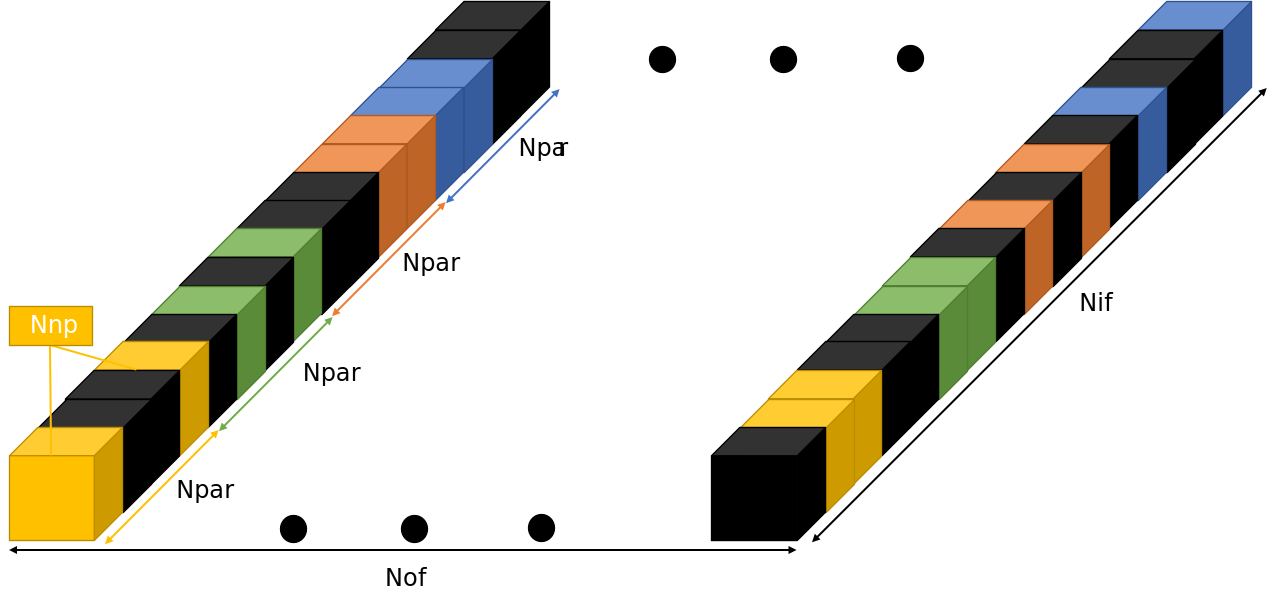
\includegraphics[width=\textwidth]{pruned_wg.pdf}
    \caption{A pointwise kernel after pruning}
    \label{fig:pruned_wg}
\end{figure}
%
After applying the pruning scheme on the pointwise kernels, the kerels become sparse and it means that is contains a lot of 0 value weights, as illustrated in Figure \ref{fig:pruned_wg}. Therefore, in order to reduce the memory usage, we should store the non-pruned weights in a compressed format that allow to find the address of the weight with no extra-overhead.

A conventional storage formats for sparse matrix is the \acrfull{csr} \cite{buluc_parallel_2009}. According to \textcite{buluc_parallel_2009}, \textquote{\textit{The compressed sparse row (CSR) format stores the nonzeros (and ideally only the nonzeros) of each matrix row in consecutive memory locations,  and  it  stores  an  index  to  the  first  stored  element of each row}}. In other words, we represent a sparse matrix using three vectors:
%
\begin{itemize}
    \item \textbf{Vector val}: containing all the values of the non-pruned weights.
    \item \textbf{Vector col\_ind}: contains the column indices of the elements in \textbf{val}.
    \item \textbf{Vector row\_ptr}: contains the index of each row in \textbf{val}.
\end{itemize}
%
However, as for \cite{zhu_efficient_2020}, this format can be compressed further thanks to the pruning scheme. Indeed, since the kernels to compress are vectors, we can reduce the storage usage by removing the \textbf{row\_ptr} vector. Moreover, we have a better compression if we reduce the number of bits allocated to represent the column index of a weigth. Indeed, knowing that the weight correpond to a pixel in a fetching group of size $N_{par}$, we can only save the position of the pixel in that group. As a result, we can reduce the number of bits from $log_2(N_{if})$ to $log_2(N_{par})$, where $N_par \leq N_{if}$.

%
\begin{figure}
    \centering
    \includegraphics[width=\textwidth]{MinCompr.pdf}
    \caption{Minimal pruning ratio if $BW$ = 16}
    \label{fig:prun_mem}
\end{figure}
%
As this compressed format requires an extra vector, we compute the minimal pruning ratio required to have a reduction of the memory usage. The relation between minimal pruning ratio and memory reduction ca be found in Equation \eqref{eq:prun_mem} where $BW$ is the bitwidth required to represent the value of a weight. The curve representing the minimal pruning ratio depending on $N_{par}$ is illustrated in Figure \ref{fig:prun_mem}. We can conclude that we need at least a pruning ration of $40\%$ in order to save memory (a fewer pruning ratio can be set if we have a small $N_{par}$).
% 
\begin{equation}
    \alpha < \frac{BW}{ BW + log_2(N_{par})}
    \label{eq:prun_mem}
\end{equation}
%
\subsection{Adding the pruning scheme to MobileNetV2}
%
As we have seen how the weights of a $1 \times 1$ kernel are pruned and the compressed format of the kernels, we explain in this section how to integrate the proposed pruning scheme into the \acrshort{dsc}. In MobileNetV2, the \acrshort{dsc} layer is included into a larger building block, the \textit{inverted residual block} (see Section \ref{subs:mbv2}). It means that the \acrshort{dsc} follows a $1 \times 1$ convolution layer that expands the number of channel. As a result, we have to compute two sparse $1 \times 1$ convolutions. 

%
\begin{figure}
    \centering
    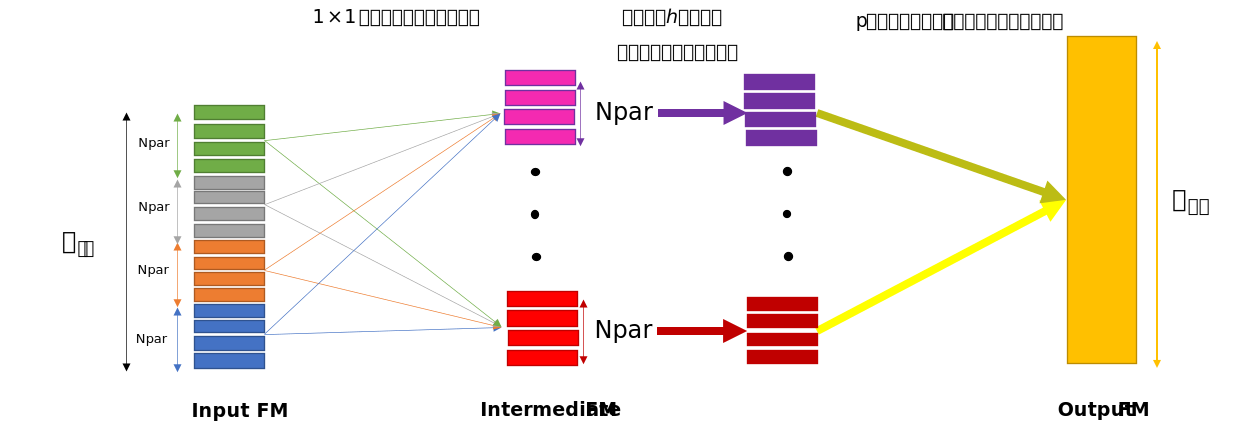
\includegraphics[width=\textwidth]{algo.pdf}
    \caption{Illustration of the algorithm used to perfom the convolutions}
    \label{fig:algo}
\end{figure}
%
As explained in Section \ref{subsec:pscheme}, each $1 \times 1$ convolution has to fetch $N_{par}$ input pixels, which corresponds to $N_{par}$ channels. Consequently, if the expansion $1 \times 1$ convolution produces $N_{par}$ channels, the \acrshort{dsc} can fetches those intermediate products and produces partial results of the output \acrshort{fm}. Indeed, we can first perform the depthwise convolution with each intermediate channel and then performing the partial pointwise convolution with the corresponding weight in each pointwise kernel, as illustrated in Figure \ref{fig:algo}. The block has finished when it has performed the previous steps for each intermediate group. This approach has been chosen, instead of producing directly each final output result, to reuse at most the products of the $1 \times 1$ convolution.

\begin{algorithm}[H]
    \centering
    \begin{algorithmic}
        \For{$group_{int}:=0$; $group_{int} < Ngr_{int}$; $group_{int}++$}
            \State{1*1\_convolution ($group_{int}$)}
            \State{DSC($group_{int}$);}
        \EndFor
    \end{algorithmic}
    \caption{Pseudocode of the algorithm}
    \label{pseudocode:overal_pseudo_code}
\end{algorithm}
%
We can translate this algorithm into a pseudocode, observed at Figure \ref{pseudocode:overal_pseudo_code}, where $group$ (respect. $group_{int}$) is the index of fetching group in the input \acrshort{fm} (resp. intermediate \acrshort{fm}, since the number of input channels is expanded by a factor $t$) and $Ngr_{int} = \left\lceil \frac{N_{if} \times t}{N_{par}} \right\rceil$ is the number of intermediate fetching group. We can now detail how each convolution is going to be performed:
%
%
\begin{enumerate}
    \item \textbf{1*1\_convolution}: We have to fetch the $N_{par}$ kernels corresponding to the \acrshort{dsc} fetching group. Indeed, the \acrshort{dsc} fetches $N_{par}$ channels corresponding to a spatial position $(intx, inty)$ of the intermediate \acrshort{fm}. Then we can perform the convolution. As described in Section \ref{subs:2dconv}, the kernel acts a sliding window on the input \acrshort{fm}. For each pixel at position $(ix, iy)$, the convolution loads iteratively each weight and pixel fetching group. For each fetching group $group \leq N_{group}$, the convolution is performed by multiplying each non-pruned weight with its corresponding channel and accumulates it with the result of the previous group. The process is finished when the $N_{par}$ intermediate \acrshort{fm} channels have been produced (of size $N_{ix} \times N_{iy}$). The corresponding pseudocode is found in Algorithm \ref{pseudocode:c11} and the process is shown in Figure \ref{fig:algo_11conv}.
    \begin{algorithm}[H]
        \centering
        \begin{algorithmic}
            \For{$int_{f}:=0$; $int_{f} < N_{par}$; $int_{f}++$} \Comment{Loop 3}
                \For{$int_{x}:=0$; $int_{x} < N_{ix}$; $int_{x}++$} \Comment{Loop 2}
                    \For{$int_{y}:=0$; $int_{y} < N_{iy}$; $int_{y}++$} \Comment{Loop 2}
                        \For{$group:=0$; $group < N_{gr}$; $group++$} \Comment{Loop 1}
                            \For{$i_f:=0$; $i_f < N_{np}$; $i_f++$} \Comment{Unrolled}
                                \State{$wgt$  = $filter_{1 \times 1}$[$group_{int} \times N_{par} + int_f$][$group \times N_{par} + i_f$]}
                                \State{$acti$  = $FMI_{I}$[$wgt[pos] + group \times N_{par}$][$int_y$][$int_x$]}
                                \State{FM$_{int}$[$group_{int} \times N_{par} + int_f$][$int_y$][$int_x$]  += $acti \times wgt[val]$}
                            \EndFor
                        \EndFor
                    \EndFor
                \EndFor
            \EndFor
        \end{algorithmic}
        \caption{Sparse $1 \times 1$ convolution pseudocode}
        \label{pseudocode:c11}
    \end{algorithm}
    %
    \begin{figure}[H]
        \centering
        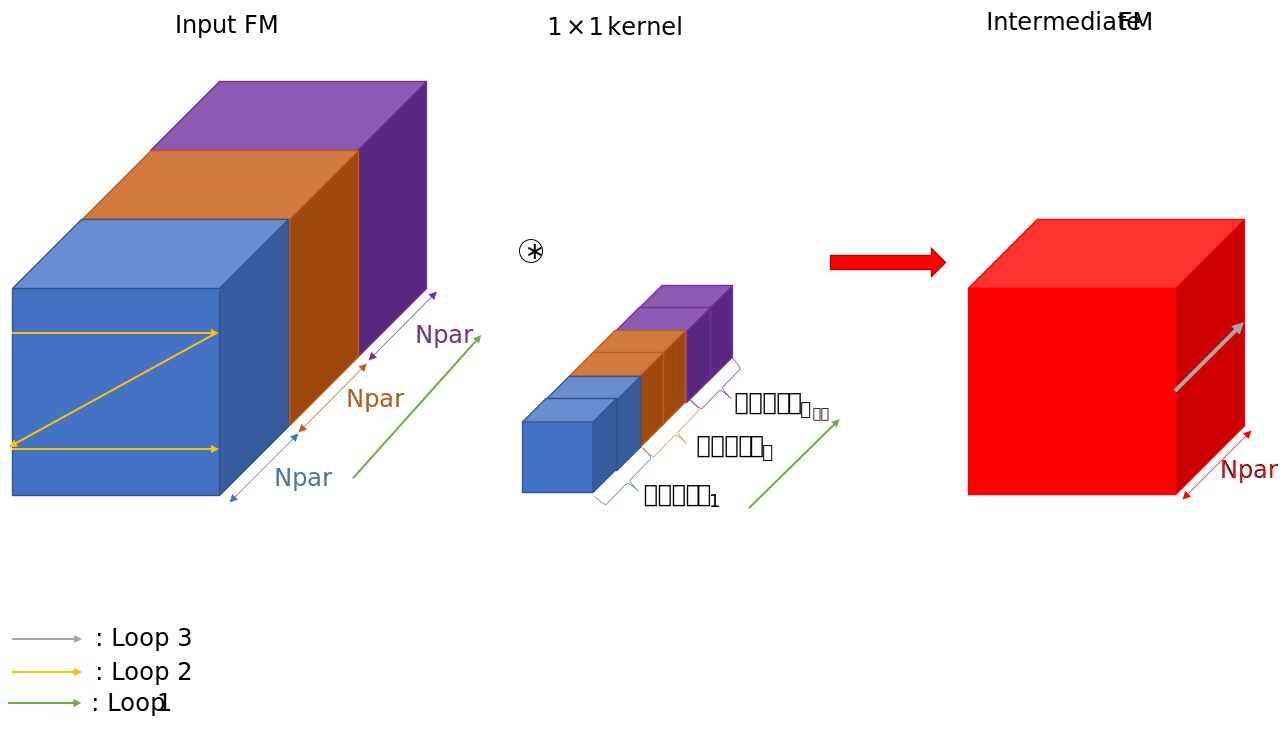
\includegraphics[width=\linewidth]{algo_c11.pdf}
        \caption{representation of the sparse $1 \times 1$ convolution}
        \label{fig:algo_11conv}
    \end{figure}
    %
    \item \textbf{\acrshort{dsc}} Once the $1 \times 1$ convolution has produced the next $N_{par}$ input channels of the \acrshort{dsc}, we can first do the depthwise convolution on the intermediate \acrshort{fm}. Once the depthwise convolution is done, we can fetch the corresponding weight fetching group in each of the pointwise filters and compute the partial results for each of the output \acrshort{fm}. The corresponding pseudocode is found in Algorithm \ref{pseudocode:dsc} and the process is shown in Figure \ref{fig:algo_dsc}.
    %
    \begin{algorithm}[H]
        \centering
        \begin{algorithmic}
            \For{$int_{f}:=0$; $int_{f} < N_{par}$; $int_{f}++$} \Comment{Loop 3}
                \For{$int_{x}:=0$; $int_{x} < N_{ix}$; $int_{x}++$} \Comment{Loop 2}
                    \For{$int_{y}:=0$; $int_{y} < N_{iy}$; $int_{y}++$} \Comment{Loop 2}
                        \For{$group:=0$; $group < N_{gr}$; $group++$} \Comment{Loop 1}
                            \For{$i_f:=0$; $i_f < N_{np}$; $i_f++$} \Comment{Unrolled}
                                \State{$wgt$  = $filter_{1 \times 1}$[$group_{int} \times N_{par} + int_f$][$group \times N_{par} + i_f$]}
                                \State{$acti$  = $FMI_{I}$[$wgt[pos] + group \times N_{par}$][$int_y$][$int_x$]}
                                \State{FM$_{int}$[$group_{int} \times N_{par} + int_f$][$int_y$][$int_x$]  += $acti \times wgt[val]$}
                            \EndFor
                        \EndFor
                    \EndFor
                \EndFor
            \EndFor
        \end{algorithmic}
        \caption{Sparse \acrshort{dsc} convolution pseudocode}
        \label{pseudocode:dsc}
    \end{algorithm}
    %
    \begin{figure}[H]
        \centering
        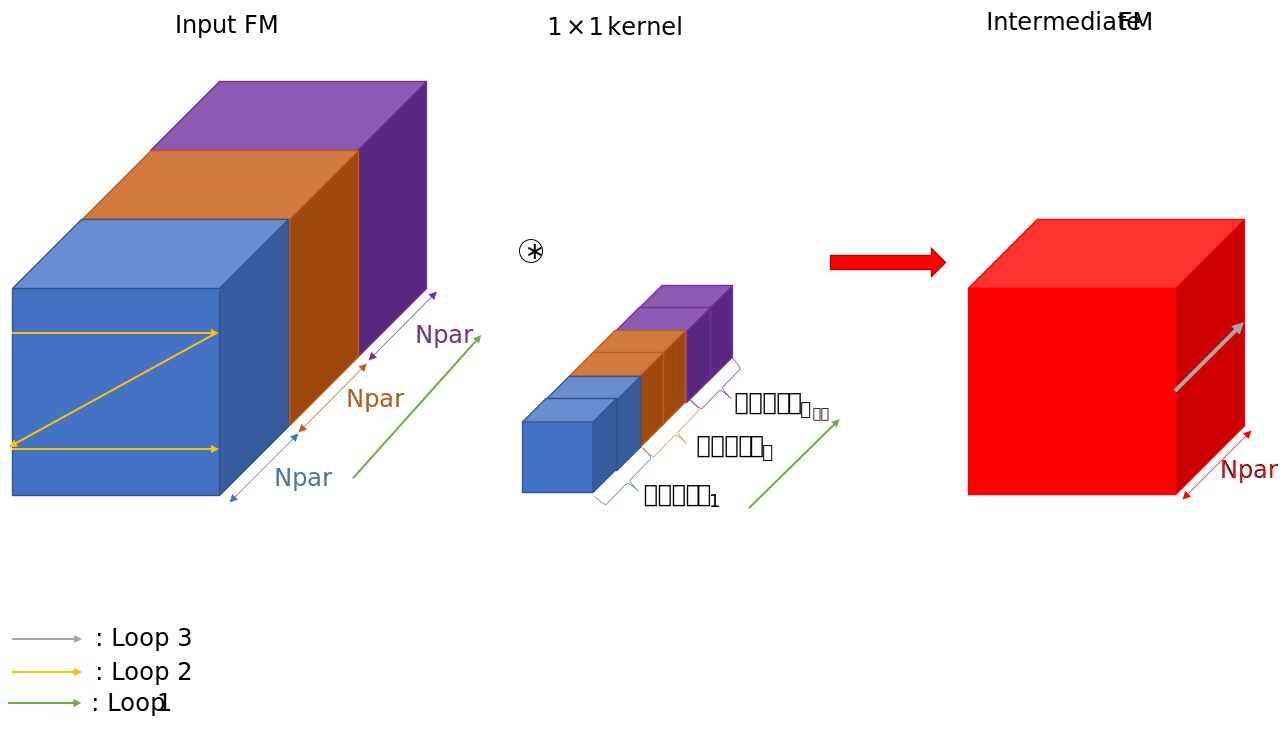
\includegraphics[width=\linewidth]{algo_c11.pdf}
        \caption{representation of the sparse \acrshort{dsc} convolution}
        \label{fig:algo_11conv}
    \end{figure}
\end{enumerate}
%
\subsection{Loop analysis}
%
Once we have determined how the convolutions is going to be performed
on \acrshort{fpga}, now we have to analyse the loop in order to find the optimal tiling, unrolling and loop interchange parameters.
%
%
\section{Implementing sparse DSC on FPGA} \label{sec:implementation}
In the previous section, we detailed how to prune $1 \times 1$ kernels, how the convolution process is performed, and we analyzed the design hardware variables. In this section, we explore how we can implement the chosen design into an \acrshort{fpga}. The hardware design was implemented using SystemVerilog and the corresponding code can be found at this address: \url{https://github.com/ggheysen/UCL-EPL-Master-Thesis-2019-2020}.

According to the scope of this thesis, the purpose of the implementation is to verify the fourth and fifth design objectives, namely:
%
\begin{itemize}
    \item The proposed architecture provides a logically correct output.
    \item An increase of the sparsity improves the performance of the architecture.
\end{itemize}
%
Those design objectives are related to the implementation of the inverted residual block with sparse $1 \times 1$ convolution. Therefore, instead of implementing each type of layer of MobileNetV2, we focus only on this one. As those two objectives are independent of the degree of parallelization, it was chosen to set all unrolling parameters to 1. We did not implement the skip connection since it is independent of the pruning scheme. However, as demonstrated by \textcite{bai_cnn_2018, liu_fpga-based_2019}, we can extend the convolution \acrshort{pe}s to support all kind of layers of MobileNetV2.

The performance results of the architecture will be discussed in next section. First, we describe the overall architecture in Section \ref{subsec:overal}, and then we go deeper into each component defined in the overall architecture. The architecture is inspired by three works: \textcite{zhu_efficient_2020, kang_accelerator-aware_2020, bai_cnn_2018}.
%
\subsection{Overall architecture} \label{subsec:overal}
%
The overall architecture has been inspired by \textcite{zhu_efficient_2020}. The mains components that compose our \acrshort{fpga}-based architecture are the following:
%
\begin{itemize}
    \item \textbf{External Memory}: it contains the \acrshort{cnn} data and it is where the output \acrshort{fm} will be stored.
    \item \textbf{Main controller}: it synchronizes the different components of the architecture by sending them control signals.
    \item \textbf{\acrfull{dma}}: it handles the read and write requests between the \acrshort{fpga} and the external memory.
    \item \textbf{\acrshort{pe}}: each \acrshort{pe} performs the actual convolution with the weight and pixel fetched from external memory into the on-chip memory. In the architecture, we have two kinds of \acrshort{pe}: $1 \times 1$ convolution \acrshort{pe} and \acrshort{dsc} \acrshort{pe}.
    \item \textbf{Buffer}: it composes the on-chip memory and contains a tile of data. There are two categories of buffer: \textbf{data buffer} which contains data from external memory and is read by the \acrshort{pe} and \textbf{result buffer} which is filled by \acrshort{pe}s and is read either by other \acrshort{pe} or by the \acrshort{dma} to write its content to external memory. There are four data buffers ($FM_{I}$ buffer, $Conv_{1 \times 1}$ buffer, $Conv_{DW}$ buffer, $Conv_{PW}$ buffer) and two result buffers ($FM_{int}$ buffer, $FM_{O}$ buffer).
\end{itemize}
%
\begin{figure}
    \centering
    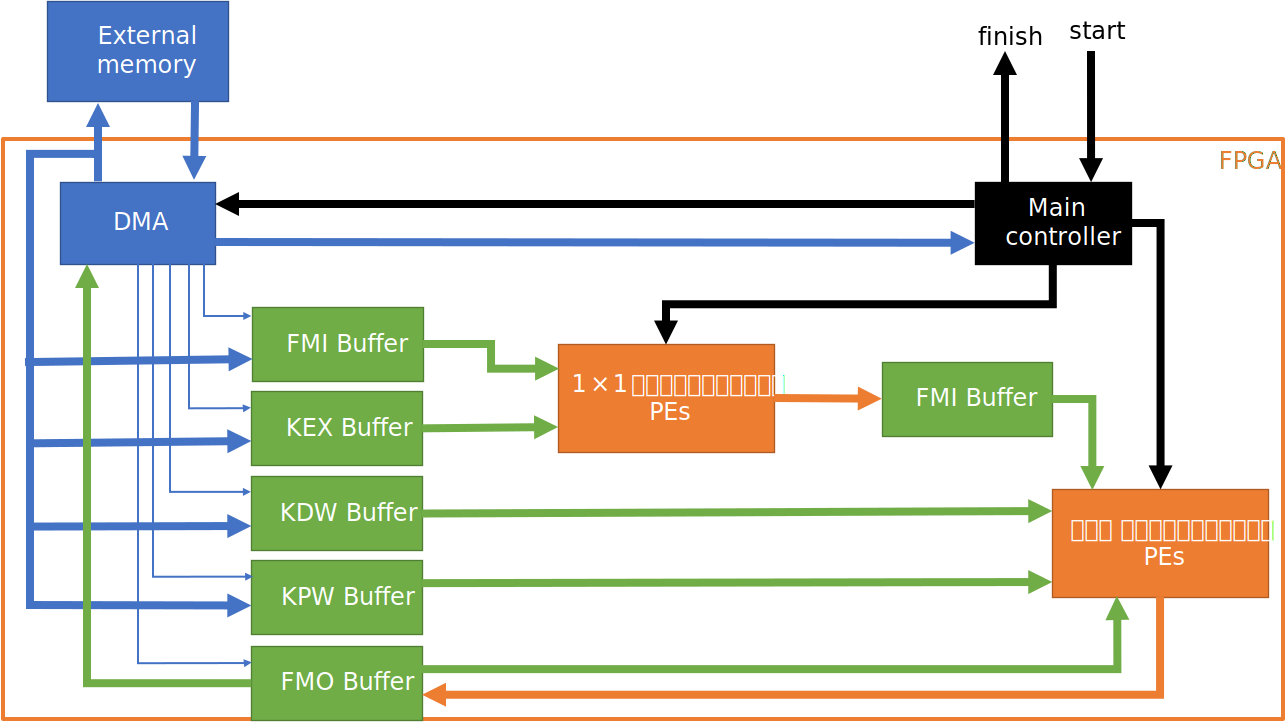
\includegraphics[width=\textwidth]{overal_archi.pdf}
    \caption{overall architecture of the accelerator}
    \label{fig:overal_archi}
\end{figure}
%
An illustration of the overall architecture can be found in Figure \ref{fig:overal_archi}. We should add that every component is synchronous with the clock signals and has reset signals. For the sake of clarity, this was not included in the drawing.

In the following sections, we will go into details about each component. An exhaustive list of the different input and output signals of each component can be found in Appendix \ref{appendix:sig}.
%
\subsection{External memory}
%
The external memory is an external component that contains all the data required to run the network (MobileNetV2) on an input \acrshort{fm}. Each data stored in the external memory can be identified by its address in the external memory. We can identify 5 types of data:
%
\begin{enumerate}
    \item \textbf{Input \acrshort{fm}}: the input \acrshort{fm} of a layer, where bitwidth representing one pixel is equal to $BW_{pixel}$. Channels are stored one by one, and the content of one channel is stored line by line. For example, the memory address of the pixel at position $\left(ix, iy, if\right)$ can be expressed using Equation \eqref{eq:addr_fmi}.
    \begin{equation}
        address_{FM_{I}}(ix, iy, if) = ix + iy \times N_{ix} + if \times N_{ix} \times N_{iy}
        \label{eq:addr_fmi}
    \end{equation}
    \item \textbf{Output \acrshort{fm}}: the output \acrshort{fm} is stored in the same manner as the input \acrshort{fm}. We should add that the output \acrshort{fm} of one layer becomes the input \acrshort{fm} of the next layer. Therefore, the addresses where the output \acrshort{fm} pixels are stored become the addresses of the input \acrshort{fm} of the next layer and inversely.
    %
    \item \textbf{$1 \times 1$ kernels}: the weights of the $1 \times 1$ convolution, where $BW_{weight}$ is the number of bits to represent the value of a weight and $log_2(N_{par})$ the number of bits to represent its position. Each $1 \times 1$ filter is stored kernel by kernel, and each kernel is stored weight by weight. For example, the memory address of the weight $x$ in fetching group \textquote{$group$} of kernel $f$ can be expressed using Equation \eqref{eq:addr_c11}.
    This terminology is used for weights from the $1 \times 1$ convolution from the bottleneck convolution and also from the $1 \times 1$ convolution layer.
    %
    \begin{equation}
        address_{K_{EX}}(kx, group, kf) = kx + group \times N_{np} + kf \times N_{np} \times N_{gr}
        \label{eq:addr_c11}
    \end{equation}
    \item \textbf{Depthwise kernels}: the depthwise kernels, where the bitwidth representing one weight is equal to $BW_{weight}$. Channels are stored one by one, and the content of one channel is stored line by line. For example, the memory address of the weigth at position $\left(kx, ky, kf\right)$ can be expressed using Equation \eqref{eq:addr_dw}.
    \begin{equation}
        address_{K_{DW}}(kx, ky, kf) = kx + ky \times N_{kx} + kf \times N_{kx} \times N_{ky}
        \label{eq:addr_dw}
    \end{equation}
    \item \textbf{Pointwise kernels}: the kernels of the pointwise convolution. The weights are stored in the same manner as for the $1 \times 1$ filter.
    \item \textbf{Standard convolution kernels}: since the first layer of MobileNetV2 is a standard convolution \cite{sandler_mobilenetv2_2019}, the weights must be also stored in the external memory, in the same manner as the depthwise filter.
\end{enumerate}

An offset, for each type of data, is added to the computation of the address to avoid that one address is shared between multiple data. As a result, before executing one layer, the main controller must have the following information, labelled as \textbf{Layer information}:
%
\begin{enumerate}
    \item \textbf{$N_{ix}$ and $N_{iy}$}: the spatial dimensions of the input \acrshort{fm}. Since $N_{ix}, N_{iy} \leq 224$ \cite{sandler_mobilenetv2_2019}, we can use 8 bits to represent them.
    \item \textbf{$N_{if}$ and $N_{of}$}: the number of channels of the input  and output \acrshort{fm}. Since $N_{if}, N_{of} \leq 1280$ \cite{sandler_mobilenetv2_2019}, we can use 11 bits to represent them.
    \item \textbf{$t$}: the expansion factor of the $1 \times 1$ convolution. Since $t \leq 6$ \cite{sandler_mobilenetv2_2019}, we can use 3 bits to represent it.
    \item \textbf{$S$}: the value of the stride. Since $S$ can be either 1 or 0 \cite{sandler_mobilenetv2_2019}, we can use 1 bit to represent it.
    \item \textbf{$N_{gr}$ and $N_{grint}$}: the number of fetching groups for the $1 \times 1$ convolution and the \acrshort{dsc}. Since the largest value possible for both parameters is the maximum $N_{if}$ ($N_{par} = 1$), we can use 11 bits to represent them.
    \item \textbf{$Layer$}: to tell the main controller which layer is going to be executed. Since there are 4 kinds of layers in MobileNetV2 \cite{sandler_mobilenetv2_2019}, we use 2 bits to represent it. However this was not included in the design because only the bottleneck convolution was implemented.
    \item \textbf{Offsets}: the offset of the different data types must be transfered to the \acrshort{dma} in order to correctly compute the address of the required data. The number of bits required to represent one offset is the bitwidth of the address of the external memory.
\end{enumerate}

%
\begin{figure}
    \centering
    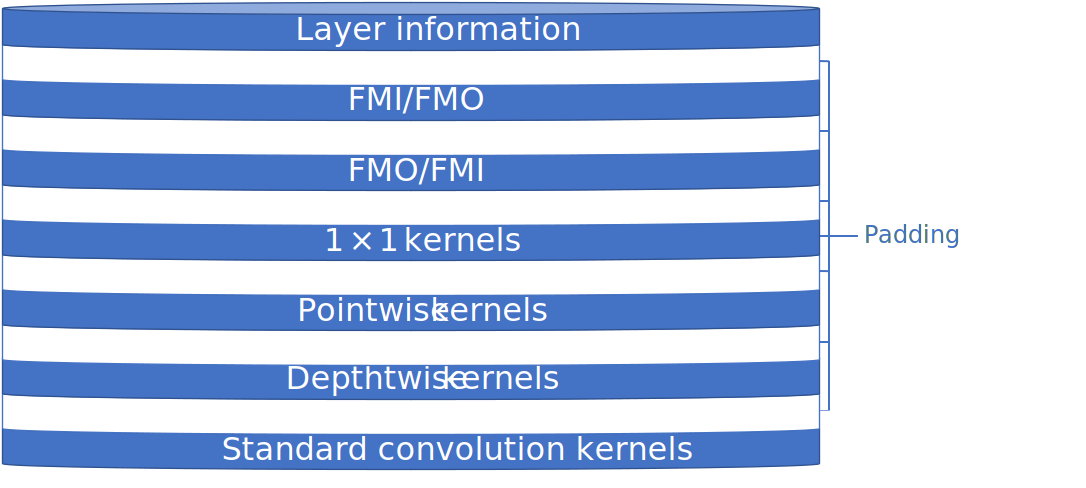
\includegraphics[width=\textwidth]{overal_mem.pdf}
    \caption{overall structure of the external memory}
    \label{fig:overal_mem}
\end{figure}
%
As a consequence, those layer information are also stored in the external memory. The overall structure of the external memory can be found in Figure \ref{fig:overal_mem}.
%
\subsection{Main controller}
%
The role of the main controller is to synchronize the different components of the architecture (except the memory components). Therefore, each component is a \textquote{slave} that stays in an idle state until the main controller wakes up one of them to perform a particular operation.

To wake up a component, the main controller sends it a starting signal $s_{*}$ and optionnaly additional information about the operation to perform. Afterwards, the main controller remains idle, waiting for the component to terminate its operation. Once the component has completed its task, it sends a finishing signal $f_{*}$ to the main controller.

The main controller remains in an idle state until it receives a starting signal indicating that the external memory contains all data to perform a bottleneck convolution. I have implemented the main controller to compute one bottleneck convolution, but its architecture could be extended to iterate through all the layers of the network.

%
\begin{figure}
    \centering
    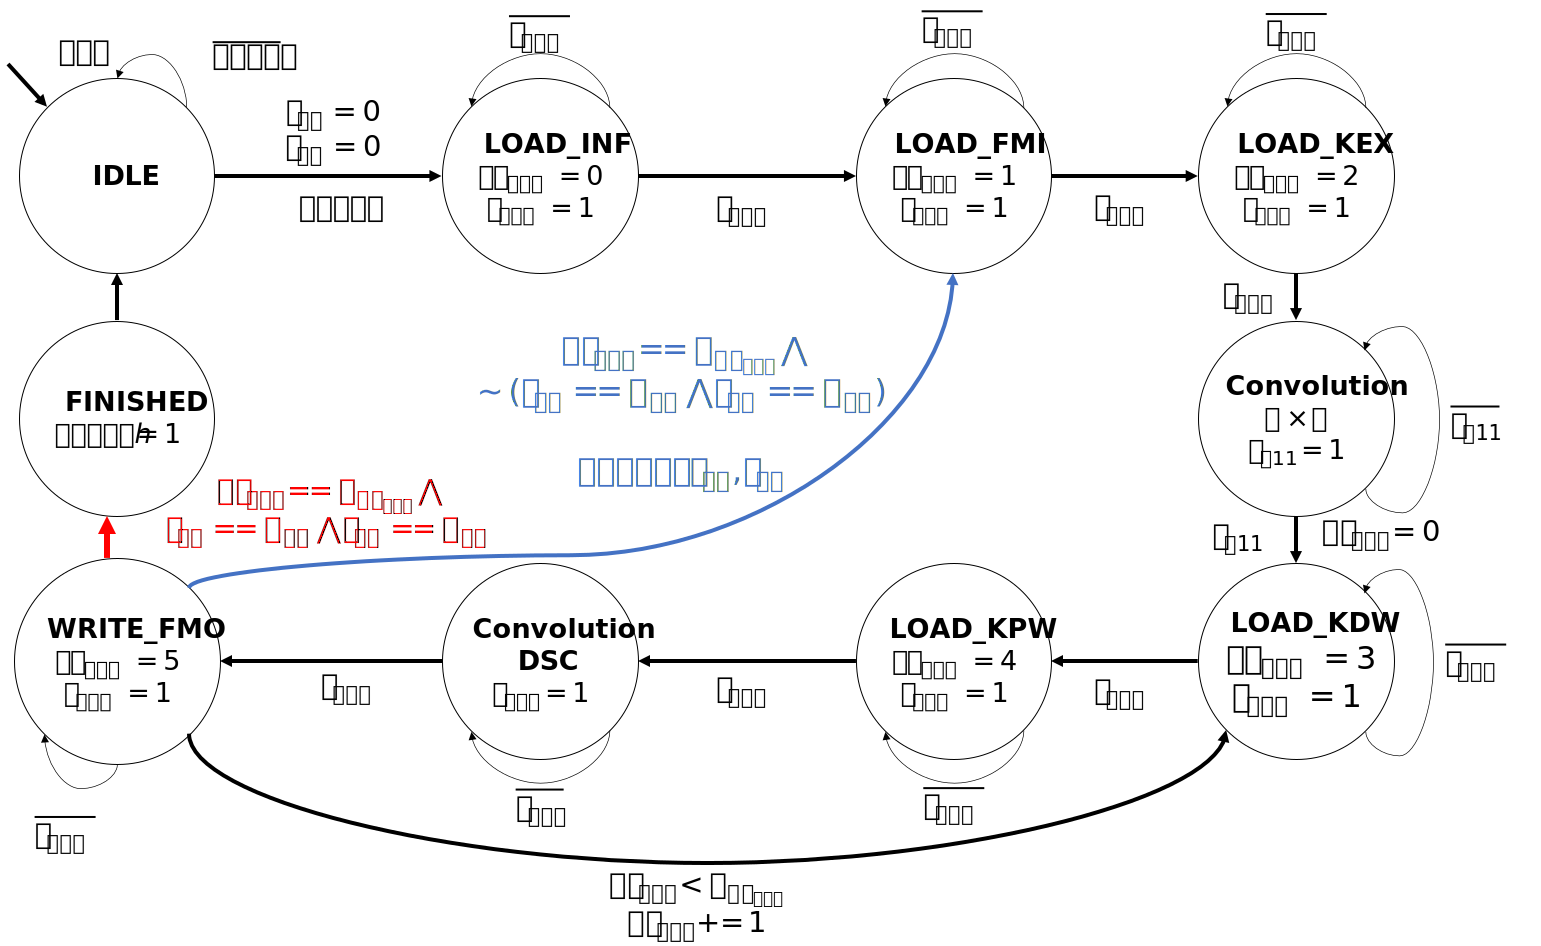
\includegraphics[width=\textwidth]{fsm-mc.pdf}
    \caption{\acrshort{fsm} of the main controller}
    \label{fig:fsm_mc}
\end{figure}
We can describe the behavior of the main controller using a \acrfull{fsm}, as illustrated in Figure \ref{fig:fsm_mc}. The \textbf{IDLE} state is the state where the main controller is waiting to perform a bottleneck convolution. Once the main controller has received a starting signal, it performs the following operations:
%
\begin{figure}
    \centering
    %
    \begin{subfigure}[t]{.49\textwidth}
        \centering
        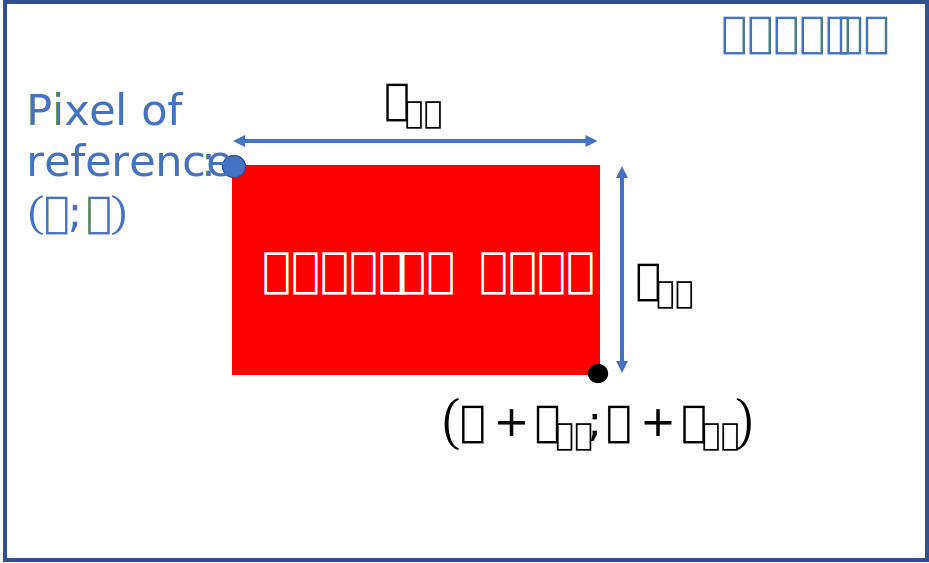
\includegraphics[width=\linewidth]{pixofref.pdf}
        \caption{Example of pixel of reference for an input \acrshort{fm} tile}
        \label{fig:pix_of_ref}
    \end{subfigure}
    %
    \begin{subfigure}[t]{.49\textwidth}
        \centering
        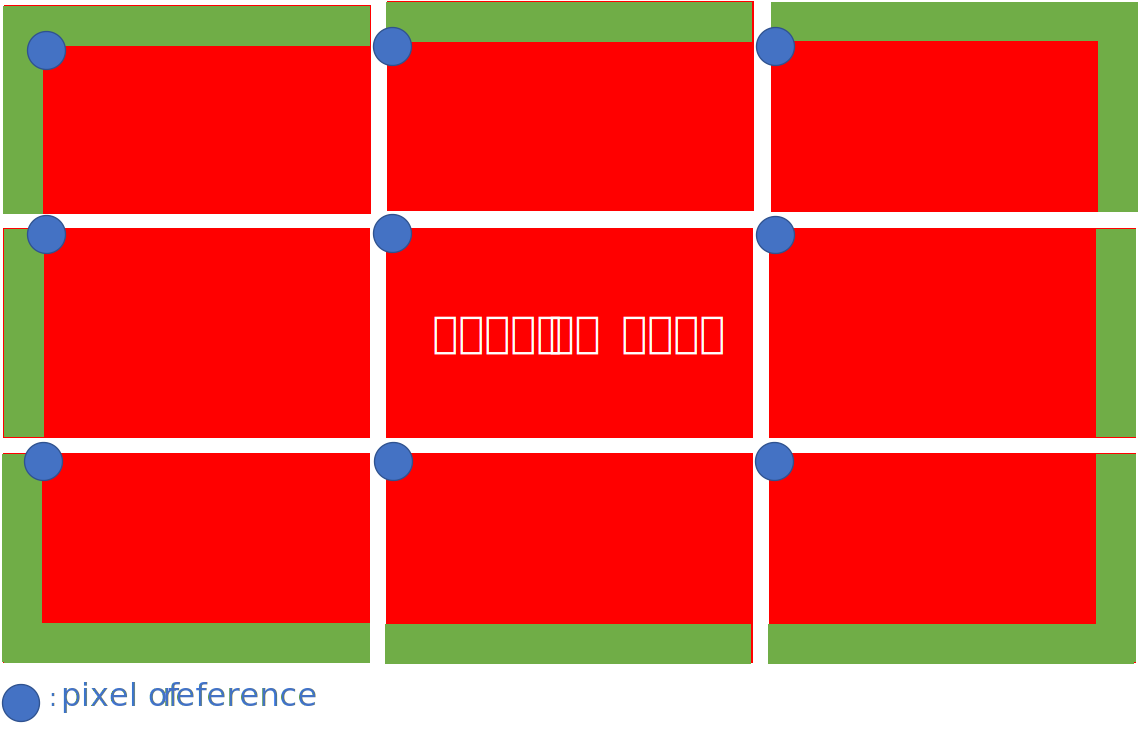
\includegraphics[width=\linewidth]{tilepadding.pdf}
        \caption{Padding configuration of input \acrshort{fm} tiles, where red area represent pixels fetched from external memory and green area represent padding pixels}
        \label{fig:tile_padding}
    \end{subfigure}
    %
    \caption{Illustration of the concept of pixel of reference and padding}
\end{figure}
%
\begin{enumerate}
    \item \textbf{LOAD\_INF}: to perform the bottleneck convolution, the main controller first needs to fetch the layer information stored in the external memory. Therefore it tells the \acrshort{dma} to fetch them.
    %
    \item \textbf{LOAD\_FMI}: the bottleneck convolution starts by fetching a tile of inputs and weights from the main memory. As all inputs in the channel-axis are buffered (corresponding to all the fetching groups), an input \acrshort{fm} tile can be determined only by the spatial coordinates of the tile first element - pixel of reference (with the smallest $(x, y)$). Indeed, the \acrshort{dma} can fetch, for each channel, all pixels in the range $[(x, y); (x+T_{ix}, y+T_{iy})]$, which corresponds to the tile, as illustrated in Figure \ref{fig:pix_of_ref}. As a result, when the main controller asks the \acrshort{dma} to load into the on-chip memory a tile of input \acrshort{fm}, it also transfers the spatial coordinates and the memory address of its pixel of reference. Moreover, since we have to add padding to the tile (spatial dimensions are not reduced by the convolution operations), 0 value pixels are stored in the on-chip memory at corresponding positions when the reference pixel is on one edge of the input \acrshort{fm}, as shown in Figure \ref{fig:tile_padding}.
    %
    \item \textbf{LOAD\_KEX}: after fetching the input \acrshort{fm} tile, the main controller asks the \acrshort{dma} to load the $N_{par}$ $1 \times 1$ kernels into the on-chip memory, corresponding to the intermediate fetching group $group_{int}$. %Rajouter le channel de ref
    \item \textbf{CONV\_11}: after loading the weights and pixels, the $1 \times 1$ convolution can be performed. Once the $N_{par}$ intermediate channels corresponding to the intermediate fetching group $group_{int}$ have been produced, the \acrshort{dsc} can be executed.
    \item \textbf{LOAD\_KDW} and \textbf{LOAD\_KPW}: before doing the \acrshort{dsc}, the pointwise and depthwise kernels corresponding to the intermediate fetching group should be loaded.
    \item \textbf{CONV\_DSC}: all output \acrshort{fm} tile partial products can be computed by performing the \acrshort{dsc} on the $N_{par}$ intermediate channels. If all intermediate fetching groups have been processed, final results are computed and can be written into the external memory. Otherwise, the next $N_{par}$ intermediate channels should be computed. Moreover, since output \acrshort{fm} partial results will be kept in on-chip memory, the main controller indicates to the \acrshort{dsc} \acrshort{pe}s whether the values read from the \textit{FMO Buffer} should be consired as valid. If it is not the case, the value should be set to 0.
    \item \textbf{WRITE\_FMO}: this state indicates that there are only final results in the \textit{FMO Buffer}. The main controller tells the \acrshort{dma} that its content can be written to the external memory. As for the input \acrshort{fm} tiles, the output \acrshort{fm} tiles are determined by their pixel of reference, which is also transmitted to the \acrshort{dma}. If all tiles have been processed, the bottleneck convolution is completed and the main controller state turns to \textbf{FINISHED}. Otherwise, a new tile has to be processed and main controller returns to \textbf{LOAD\_FMI} state.
    \item \textbf{FINISHED}: The bottleneck convolution is done and the main controller sets the finish signal.
\end{enumerate}
%
\subsection{DMA}
%
The purpose of the \acrshort{dma} is to fill the \textbf{data buffer} with its corresponding tile fetched from external memory and write the output pixels into the external memory. Therefore, it has to manage six types of operation, referenced by its operation number $op_{dma}$:
%
\begin{itemize}
    \item $op_{dma} = 0$: Load the layer information
    \item $op_{dma} = 1$: Load an input \acrshort{fm} tile, referenced by its pixel of reference. The \acrshort{dma} needs as extra information the coordinate and the memory address of that pixel of reference.
    \item $op_{dma} = 2$: Load the $1 \times 1$ kernels used to produce the intermediate fetching group $group_{int}$ of size $N_{par}$. The \acrshort{dma} needs as extra information the first kernel and the memory address of its first weight to correctly load the $N_{par}$ kernels.
    \item $op_{dma} = 3$: Load the depthwise kernels corresponding to the intermediate fetching group $group_{int}$ of size $N_{par}$. The \acrshort{dma} needs as extra information the first kernel of the group and the memory address of its first weight to correctly load the $N_{par}$ kernels.
    \item $op_{dma} = 4$: Load the weight fetching group (of size $N_{np}$) of all pointwise kernels corresponding to the intermediate fetching group $group_{int}$. The \acrshort{dma} needs as extra information the position of the first weight in the fetching group and its memory address.
    \item $op_{dma} = 5$: Write the content of the \textbf{FMO Buffer} into the external memory, which corresponds to a tile of output \acrshort{fm}. As this tile is referenced by its pixel of reference, the \acrshort{dma} needs as extra information the coordinate and the memory address of that pixel of reference.
\end{itemize}

%
\begin{figure}
    \centering
    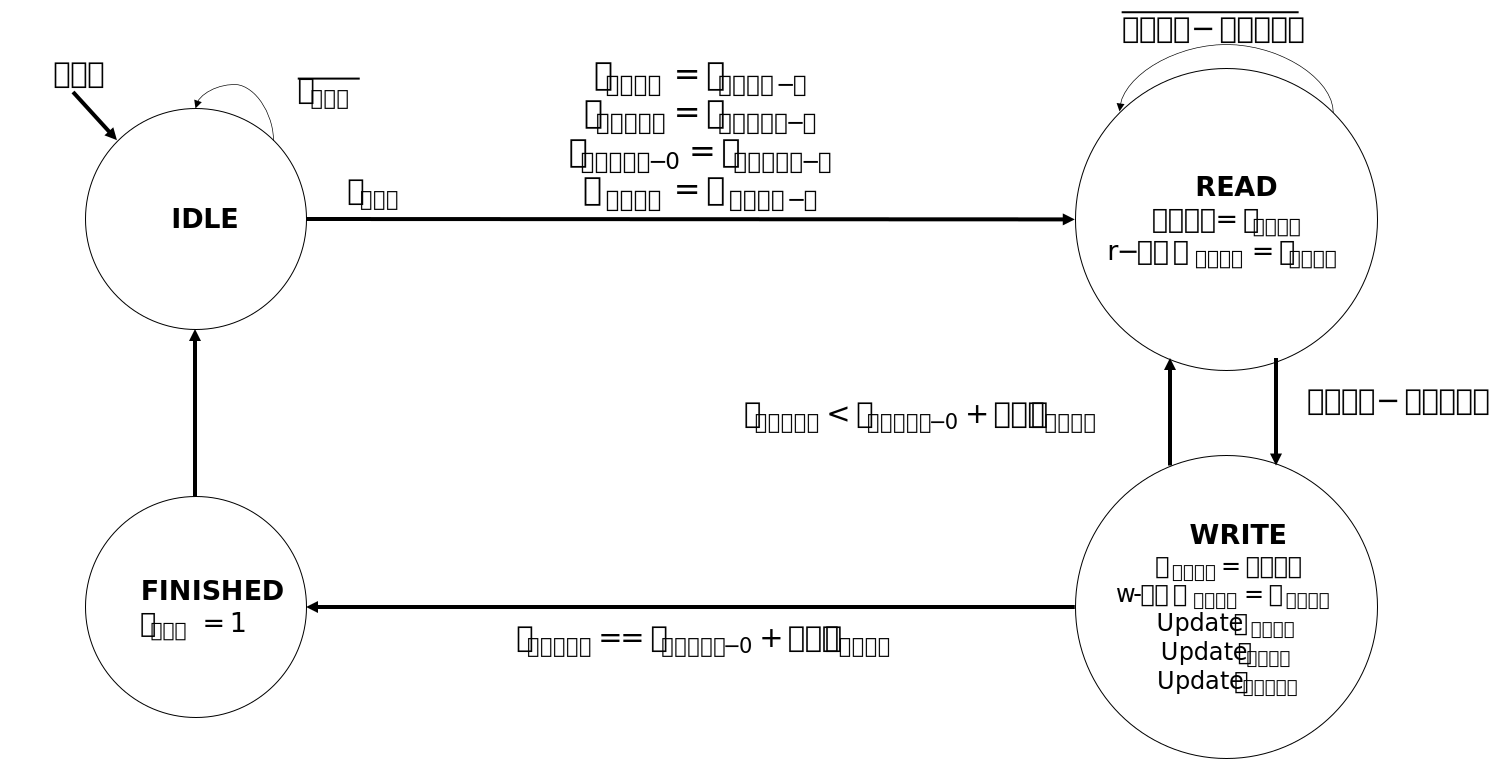
\includegraphics[width=\textwidth]{fsm-dma.pdf}
    \caption{\acrshort{fsm} of the \acrshort{dma}}
    \label{fig:fsm_dma}
\end{figure}
When the main controller asks the \acrshort{dma} for a transfer, it sets its start signal, which operation to execute ($op_{dma}$), and all extra information required. All extra information are related to the external memory, if the \acrshort{dma} reads or writes into a buffer, the initial address $r_{addr-i}/w_{addr-i}$ can be set to 0. The behavior of the \acrshort{dma} can be expressed using a \acrshort{fsm}, as found in Figure \ref{fig:fsm_dma}. A general \acrshort{fsm} has been illustrated because each operation shares the same structure. As the \acrshort{dma} only fetches data from one memory and writes the data into another one, each operation is composed of 2 states:
\begin{itemize}
    \item \textbf{READ}: the \acrshort{dma} fetches the required data at a address $r_{addr}$. Once the data is loaded by the \acrshort{dma}, it moves to the next state to write the data in the on-chip memory. When loading the input \acrshort{fm} tile, if the address corresponds to a padding pixel, the value to write is 0 and the \acrshort{dma} directly moves to the \textbf{WRITE} state. If the data is fetched from the external memory, the \acrshort{dma} waits the data read from the external memory to be valid. But if the data is fetched from a buffer, the process can be pipelined. That is why, before the \acrshort{dma} reads data from the on-chip memory, it is in a state called \textbf{RAM\_LOADING} to initialize the pipeline process.
    \item \textbf{WRITE}: the \acrshort{dma} sends a write signal and the associated data $w_data$ and address $w_{address}$ to the corresponding memory . If the operation is finished (the tile has been fetches), the \acrshort{dma} goes into the \textbf{FINISHED} state. Otherwise, it updates the address of the next data to fetch and goes back to the \textbf{READ} state.
\end{itemize}

Since the \acrshort{dma} performs one transfer at a time, we can share the fetched data (to be written) $w_{data}$ between all memory component and we set the write signal to the corresponding component. In a similar way, the signal to access or write data in a buffer $ram_{addr}$ can also be shared between the different buffers.
%
\subsection{1\texttimes1 convolution PE}
%
The purpose of this component is to execute the Algorithm \ref{fig:algo_11conv}. The behavior of the \acrshort{pe} can be expressed using a \acrshort{fsm}, as found in Figure \ref{fig:fsm_c11}.

When the \acrshort{pe} receives a starting signal, it means that the \textbf{FMI} and \textbf{KEX BUFFERS} contain the data to execute the next $1 \times 1$ convolution. For each fetching group corresponding to an intermediate pixel at address $\left( int_x, int_y, int_f \right)$, the \acrshort{pe} loads the corresponding inputs and weights into its registers (\textbf{LOAD\_DATA} state). Once it is done, the computation can be performed (\textbf{COMPUTATION} state). Since the convolution is fully-unrolled, an exemple of the hardware configuration is shown in Figure \ref{fig:c11_hardware}. The output result is then summed with the content of the accumulator (which contains 0 for the first fetching group).

When the convolution is done for one intermediate pixel, the result is written into the \textbf{FMINT BUFFER}. If all pixels required for the \acrshort{dsc} have been computed, the \acrshort{pe} sends an ending signal to the main controller (\textbf{FINISHED} state). Otherwise it computes the next intermediate pixel.
%
\subsection{DSC PE}
%
This \acrshort{pe} is designed to perform the \acrshort{dsc}. Once the $1 \times 1$ convolution has computed the next \acrshort{dsc} fetching group and the \textbf{Buffers} containts the required data, we can do the \acrshort{dsc} as in Algorithm \ref{fig:algo}. The \acrshort{pe} can be described as a \acrshort{fsm} executign Algorithm \ref{fig:algo_dsc}.
%
\subsection{Buffer}
%
\begin{figure}
    \centering
    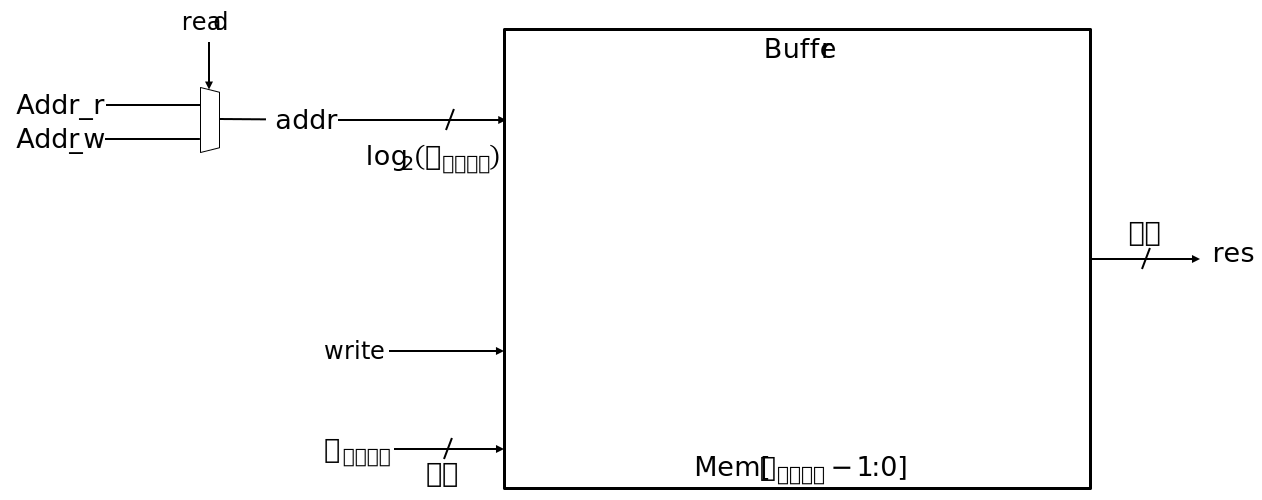
\includegraphics[width=\textwidth]{struct_ram.pdf}
    \caption{General architecture of a buffer component}
    \label{fig:struct_ram}
\end{figure}
%
The buffers compose the on-chip memory of the \acrshort{fpga}. As mentionned previously, the structure is composed of six buffers that share the same structure, as illustrated in Figure \ref{fig:struct_ram}. At each clock period, the output signal $res$ is equal to the value stored at address $addr$, or if the write signal $write$ is enabled, the value that is currently written. In the same way, if the write signal is set, the value in the buffer at address $addr$ is equal to the input data $w_{data}$. As multiple components may read or write a same buffer, a multiplexer is added to select from which address to read.

The value of $addr_r$ and $addr_w$ depend on the type of buffer. For \textbf{data buffer} the $addr_r$ is the \acrshort{pe} address of the corresponding buffer, and $addr_w$ is the \acrshort{dma} $ram_{addr}$ signals. For \textbf{result buffer}, $addr_w$ is the corresponding \acrshort{pe} output address and $addr_r$ can be either a \acrshort{pe} address requesting a result (\textbf{FMINT Buffer}) or the \acrshort{dma} $ram_{addr}$ signals to write final results to external memory ((\textbf{FMO Buffer}))

However, the differences between each buffer are the maximum number of elements that can be stored $N_{elem}$ and the bitwidth $BW$ of their data stored. We explore for each buffer these two parameters.
\begin{itemize}
    \item \textbf{FMI Buffer}: we have determined from the loops analysis that we buffer each input \acrshort{fm} fetching group. Since the number of input \acrshort{fm} channels vary accross the different layers of the network, we can determine $N_{elem}$ using Equation \eqref{eq:nelem-fmi}. The number of bits to store a pixel is equal to $BW_{pixel}$. We can therefore express $BW$ such as Equation \eqref{eq:bw-fmi}.
    \begin{equation}
        N_{elem-fmi} = \forall l \in layers: Max\left( N_{if}^l \times Min\left(T_{ix}, N_{ix}^l\right) \times Min\left(T_{iy}, N_{iy}^l\right) \right)
        \label{eq:nelem-fmi}
    \end{equation}
    \begin{equation}
        BW_{fmi} = BW_{pixel}
        \label{eq:bw-fmi}
    \end{equation}
    %
    \item \textbf{KEX Buffer}: this buffer stores the $N_{par}$ $1 \times 1$ kernels required to perform this convolution, which expands the number of input channels. Therefore, we can express $N_{elem}$ using Equation \eqref{eq:nelem_kex}, where $N_{gr-max} = \left\lceil \frac{1280}{Npar} \right\rceil$ is the maximum number of fetching group in the whole network. Since the weights are expressed in the proposed compressed format, we also have to store the weight position in the fetching group.
    As a result, $BW$ can be expressed using Equation \eqref{eq:bw-kex}, where $BW_{weight}$ is the number of bits to represent a weight and $log_2(N_{par})$ the number of bits to represent the position.
    \begin{equation}
        N_{elem-kex} = N_{par} \times N_{np} \times N_{gr-max}
        \label{eq:nelem_kex}
    \end{equation}
    \begin{equation}
        BW_{kex} = BW_{weight} + log_2(N_{par})
        \label{eq:bw-kex}
    \end{equation}
    %
    \item \textbf{FMINT Buffer}: since the \acrshort{dsc} needs $N_{par}$ intermediate \acrshort{fm} channels and the $1 \times 1$ convolution does not reduce the spatial dimension of the input \acrshort{fm}, we can express the $N_{elem}$ using Equation \eqref{eq:nelem_fmint}. The bitwidth of a pixel is the bitwidth used to represent a pixel, as in Equation \eqref{eq:bw-fmint}.
    \begin{equation}
        N_{elem-fmint} = N_{par} \times T_{iy} \times T_{ix}
        \label{eq:nelem_fmint}
    \end{equation}
    \begin{equation}
        BW_{fmi} = BW_{pixel}
        \label{eq:bw-fmint}
    \end{equation}
    %
    \item \textbf{KDW Buffer}: applying the same methodoly as \textbf{FMINT Buffer} and since the depthwise kernels are fully buffered, we can express the $N_{elem}$ using Equation \eqref{eq:nelem_kdw}. The bitwidth of a pixel is the bitwidth used to represent a weight, as in Equation \eqref{eq:bw-kdw}.
    \begin{equation}
        N_{elem-kdw} = N_{par} \times N_{ky} \times N_{kx}
        \label{eq:nelem_kdw}
    \end{equation}
    \begin{equation}
        BW_{kdw} = BW_{weight}
        \label{eq:bw-kdw}
    \end{equation}
    %
    \item \textbf{KPW Buffer}: for each time we perform a \acrshort{dsc}, we need to convolve in each pointwise the corresponding weight fetching group with $N_{np}$ pixels in the $N_{par}$ channels. The maximum number of elements in the buffer can be computed using Equation \eqref{eq:nelem_kpw}. As the pointwise convolution is a $1 \times 1$ convolution, the bitwidth associated to each pointwise kernel is the same as the \textbf{KPW Buffer}, and can be expressed using Equation \ref{eq:bw-kpw}
    \begin{equation}
        N_{elem-kpw} = N_{np} \times N_{of}
        \label{eq:nelem_kpw}
    \end{equation}
    \begin{equation}
        BW_{kpw} = BW_{weight} + log_2(N_{par})
        \label{eq:bw-kpw}
    \end{equation}
    %
    \item \textbf{FMO Buffer}: using the same methodoly as for determining $N_{elem}$ and $BW$ for the \textbf{FMI Buffer}, they are expressed using Equation \eqref{eq:nelem_fmo} and \eqref{eq:bw_fmo}
    \begin{equation}
        N_{elem-fmo} = \forall l \in layers: Max\left( N_{of}^l \times Min\left(T_{oy}, N_{oy}^l\right) \times Min\left(T_{ox}, N_{ox}^l\right) \right)
        \label{eq:nelem_fmo}
    \end{equation}
    \begin{equation}
        BW_{fmo} = BW_{pixel}
        \label{eq:bw_fmo}
    \end{equation}
\end{itemize}

%

%
%
\chapter{Measure and Results}
blabla
%
%
\newpage

	
	%% Conclusion
	\chapter{Conclusion} \label{chap:ccl}
This works is very good.
\section{Future Works}
It is perfect.
\afterpage{\blankpage}
\newpage

  	
  	%% Bibliography
	\input{src/0.Bibliography/Bibliography}
  	% Back cover page
  	\backcoverpage

\end{document}
